% =====================================================================
%  CALM -- JRSS Series B manuscript.  Built 2026-09-04 from results/*.csv (see AI_BRAIN.md).
%  Compile: pdflatex paper.tex (x2).  RSS house style: numbered headings, no bullets, no footnotes,
%  theorems numbered by type, matrices ITALIC / vectors BOLD, exp not e, abstract <= 200 words,
%  5-6 alphabetical keywords each in the abstract, alt text under every figure.
%  Every number below traces to a file in results/ named in AI_BRAIN.md; do not edit a number here
%  without editing the source of truth.
% =====================================================================
\documentclass[namedate,webpdf,modern,mediumone]{oup-authoring-template}

\usepackage{amsmath,amssymb}
\usepackage{graphicx}
\usepackage{booktabs}

\newcommand{\societylogo}{}
\graphicspath{{Fig/}}

\DeclareMathOperator{\var}{var}
\DeclareMathOperator{\tr}{tr}
\DeclareMathOperator{\expit}{expit}
\newcommand{\adist}{\mathrel{\dot\sim}}
% RSS convention: matrices ITALIC upper case, vectors BOLD
\newcommand{\bb}{\boldsymbol{\beta}}
\newcommand{\bbh}{\hat{\boldsymbol{\beta}}}
\newcommand{\bbt}{\tilde{\boldsymbol{\beta}}}
\newcommand{\by}{\boldsymbol{y}}
\newcommand{\bpi}{\boldsymbol{\pi}}
\newcommand{\br}{\boldsymbol{r}}
\newcommand{\bv}{\boldsymbol{v}}
\newcommand{\bmu}{\boldsymbol{\mu}}
\newcommand{\bx}{\boldsymbol{x}}
\newcommand{\bpsi}{\boldsymbol{\psi}}
\newcommand{\Om}{\Omega}

\theoremstyle{thmstyleone}
\newtheorem{theorem}{Theorem}
\newtheorem{proposition}{Proposition}
\newtheorem{lemma}{Lemma}
\theoremstyle{thmstyletwo}
\newtheorem{elaw}{Empirical relation}
\theoremstyle{thmstyleone}
\newtheorem{corollary}{Corollary}
\theoremstyle{thmstyletwo}
\newtheorem{remark}{Remark}
\theoremstyle{thmstylethree}
\newtheorem{assumption}{Assumption}

\begin{document}

\journaltitle{Journal of the Royal Statistical Society Series B}
\DOI{}
\copyrightyear{2026}
\pubyear{2026}
\vol{00}
\issue{0}
\access{}
\appnotes{Paper}
\firstpage{1}

\title[Goodness-of-fit reference under shrinkage]{A closed-form goodness-of-fit reference for
penalised logistic regression in the proportional regime}

\author[1,$\ast$]{Ebrahim Khaled Ebrahim}

\address[1]{\orgdiv{Department of Applied Statistics},
\orgname{Alexandria University}, \orgaddress{\country{Egypt}}}

\corresp[$\ast$]{Corresponding author. Department of Applied Statistics, Faculty of Business,
Alexandria University, Alexandria 5424074, Egypt.
\href{mailto:ebrahimkhaled@alexu.edu.eg}{ebrahimkhaled@alexu.edu.eg}}

% RSS: <= 200 words, NO citations, no abbreviations; every keyword must appear here.
\abstract{Grouped goodness-of-fit tests for logistic regression, such as the Hosmer--Lemeshow
test, assume maximum likelihood fitting. Under ridge regression, shrinkage displaces the grouped residuals, and removing it leaves a first-order
reference that is conservative. The residuals are standardised by the fitted Bernoulli variance,
which shrinkage inflates towards one quarter; the resulting deflation removes 19 per cent of the
statistic when predictors are a quarter of the sample, and any residual diagnostic standardised by
a fitted variance inherits the error. Evaluating the variance at the debiased fit makes the
reference asymptotically exact at fixed dimension. In the proportional regime of high-dimensional
logistic regression we estimate the null variance from one fit by the observable adjustments of
regularised M-estimation, and identify the remaining term as response-dependent grouping. The
resulting test of calibration along the fitted index, CALM, needs no resampling: on a smooth basis
whose degree adapts to an observable measure of index noise it matched the bootstrap in power and
never exceeded its level up to aspect ratio 0.4 in every design with balanced outcomes. The decile
basis needs a calibrated correction that does not transfer, and neither basis survives strongly
unbalanced outcomes at those ratios. An R implementation is provided.}

\keywords{calibration; goodness-of-fit; high-dimensional logistic regression; Hosmer--Lemeshow
test; proportional regime; ridge regression}

\maketitle

% =====================================================================
\section{Introduction}\label{sec:intro}
% =====================================================================

Penalised logistic regression is widely used to build a clinical prediction model
when the number of candidate predictors is large relative to the number of events
\citep{riley2021,pavlou2024}, and the fitted model is then checked for calibration in the usual
way, almost always with a grouped goodness-of-fit test such as the Hosmer--Lemeshow test
\citep{hosmer1980,hosmer1997}. This combination is not valid. Under a ridge penalty the grouped standardised residuals acquire a
non-centrality induced by shrinkage, and at the penalty that cross-validation selects the test
rejects correctly specified models between 92 and 100 per cent of the time
\citep{ebrahim2026seriesc}. Subtracting an estimate of the shrinkage displacement removes that
non-centrality and restores the ordinary maximum likelihood covariance to first order, but the
first-order reference distribution it restores is itself wrong: it is conservative, and
increasingly so as the ratio of predictors to observations grows, so that until now a valid test
could be had only by prepivoting \citep{beran1987,beran1988} --- which Section~\ref{sec:sim} shows
also loses its level at the top of the range treated here --- a bootstrap in which the penalised
model is refitted in every resample. The defect is in the standardisation itself, and it is not
confined to grouped tests.

The explanation is simple once seen. The
grouped residuals are standardised by the Bernoulli variance $\hat\pi_i(1-\hat\pi_i)$ evaluated
at the \emph{fitted} probabilities. Ridge regression pulls every fitted probability towards one
half, where $\pi(1-\pi)$ is largest, so the standardisation uses a variance that is too large and
every residual looks smaller than it is. The error is of order $\lambda/n$, where $\lambda$ is the
penalty and $n$ the sample size; it is negligible in the asymptotic regime of the first-order
theory and material at the penalties analysts actually use --- 7 per cent of the statistic at
$\lambda/n = 0.2$ and 19 per cent when the number of predictors is a quarter of the sample size.
Evaluating the variance at the debiased fit instead makes the analytic reference asymptotically
exact wherever the first-order theory applies. The point is not confined to grouped tests. Every residual
diagnostic for a penalised generalised linear model that standardises a residual by its fitted
variance divides by a quantity that shrinkage has moved towards the maximum of the variance
function, and so reports a statistic that is systematically too small; Pearson-type and
deviance-type statistics for penalised fits should show the same error.

In the proportional regime, where $p/n \to \kappa \in (0,1)$, two further things happen, and
both are dealt with here. First, the debiased fit is itself noisy, so its Bernoulli variance
understates the truth; we use the observable adjustments of \citet{bellec2022} for regularised
M-estimation to estimate the null variance from the fit alone. Second, grouping on a noisy fitted
index selects observations by their own noise, which leaves a non-centrality in the corrected
residual. We show that this term is of order $\kappa$ within a design family, that under
balanced outcomes it is concentrated almost entirely in the cubic direction of the group index, and
that it is then removed by a basis whose polynomial degree is chosen from an observable measure of
index noise --- a rule that the attenuation law of
\citet{ebrahim2026seriesc} already recommends on grounds of power. The result is a test with a closed-form reference distribution and no resampling. We call it CALM, for calibration assessment under lambda-shrunk models; the name records what the
statistic is computed from and where, and Section~\ref{sec:corrected} states precisely which
hypothesis it tests, which is not the calibration of the shrunk probabilities themselves. One conclusion deserves to be stated at the
outset, because it decides the design: in the proportional regime the choice of basis is not a
matter of taste but of validity. A basis that spends every group direction cannot avoid the
direction the selection term occupies, and can only absorb it into the reference through a constant
that must be calibrated; a basis of low polynomial degree can leave that direction out, and then no
constant is needed. The EDGE basis of \citet{ebrahim2026edge}, introduced there to direct a test at
the departures a calibration curve can show, turns out to be the ingredient that makes an
untuned closed-form reference possible here. Tests for high-dimensional regression built by other routes --- the residual prediction tests of \citet{shah2018} for linear models and \citet{jankova2020} for generalised linear models, and the coefficient tests of \citet{guo2016} --- ask whether the model is correct as a function of the covariates, or whether a block of coefficients is zero; the statistics treated here ask whether the
deployed predictor is calibrated along its own index, and Section~\ref{sec:power} shows that the two families reject on essentially disjoint datasets:
against an omitted interaction off the index the residual prediction test rejects $0.877$ at fixed
$p$ where CALM rejects $0.058$, and against a departure along the index the ordering reverses. The
present paper supplies the analytic reference that the second family lacked.

It is worth saying at the outset what a test of this kind can and cannot deliver. The ideal is
validity at any aspect ratio together with power against every departure from the logistic form,
and that ideal is out of reach for any test built on the fitted index. Grouping on a noisy index
attenuates a departure of degree $k$ by $\rho^{2k}$, where $\rho$ is the correlation between the
fitted and the true linear predictor (Proposition~\ref{prop:atten}), and $\rho$ is about $0.7$ at
$\kappa = 0.25$, so a cubic departure arrives with about a tenth of its non-centrality and no
grouped test on that index can find it, whatever reference it uses. What is attainable, and what
this paper delivers, is a valid reference computed from a single fit together with power against
the departures the index preserves. Section~\ref{sec:boundary} shows that a bootstrap with $399$
refits reaches no further.

The contributions are as follows. (a) Theorem~\ref{thm:variance} identifies the fitted-variance deflation and gives the corrected
first-order law. (b)
Proposition~\ref{prop:denoised} gives an observable estimate of the null variance in the
proportional regime, and Section~\ref{sec:selection} characterises the selection non-centrality,
its order in $\kappa$ and its cubic structure. (c) Corollary~\ref{cor:adaptive} turns the attenuation law of
\citet{ebrahim2026seriesc}, restated here as Proposition~\ref{prop:atten}, into an adaptive basis
that retains the directions in which a departure survives grouping and, as a consequence, removes
the selection term. (d) Section~\ref{sec:sim} separates the two bases: on the adaptive EDGE basis, which by
construction avoids the direction the selection term occupies, CALM held or fell below its level in all twenty-five balanced designs of
Tables~\ref{tab:sizeA} and~\ref{tab:heldout}, for $\kappa$ up to $0.4$ and for three predictor laws, while on the decile basis it needs the calibrated correction; we report
the designs in which that correction is too small, and the unbalanced designs in which neither basis
holds its level. (e) Section~\ref{sec:power} compares CALM with prepivoting, with the
high-dimensional test of \citet{jankova2020} and with the calibration checks in clinical use, which
do not hold their level on a penalised fit.

Three kinds of statement follow, and we keep them apart throughout.
Theorem~\ref{thm:variance} is proved here, and Corollary~\ref{cor:adaptive} follows from the
attenuation law of \citet{ebrahim2026seriesc}, restated as Proposition~\ref{prop:atten}.
Proposition~\ref{prop:denoised} rests on the theorems of \citet{bellec2022} under a Gaussian design
and on the consistency of a one-dimensional scale estimate, which we assume. The relation of
Section~\ref{sec:selection} that supplies the inflation factor is fitted on eight simulation cells
and is not derived: Section~\ref{sec:heldout} reports its behaviour in sixteen cells that did not
calibrate it, including five in which the decile statistic fails. The statistic we recommend, on
the adaptive basis of Corollary~\ref{cor:adaptive}, does not depend on that constant wherever the
rule takes degree two, which it did in every proportional-regime cell we examined: the inflation it
applies is then inert, at most $1.05$. Where the index
is accurate enough for the rule to keep the cubic, as on the data of Section~\ref{sec:glaucoma}, the
constant returns.

Section~\ref{sec:setup} sets out the shrinkage-corrected statistics and the first-order law we take
as given, Section~\ref{sec:variance} proves the fitted-variance deflation, Section~\ref{sec:prop}
builds the observable reference in the proportional regime and defines CALM,
Section~\ref{sec:sim} reports the numerical study, Section~\ref{sec:glaucoma} returns to the
glaucoma data of \citet{ebrahim2026seriesc}, and Section~\ref{sec:disc} states what is proved, what
is calibrated and where the boundary lies. The proofs are short and are given where the results are
stated; the behaviour of the correction under penalties other than the ridge is reported in the
online supplementary material.

% =====================================================================
\section{The shrinkage-corrected statistics and their first-order law}\label{sec:setup}
% =====================================================================

\subsection{Notation}\label{sec:notation}

Let $y_i \in \{0,1\}$ and $\bx_i \in \mathbb{R}^{p}$, $i = 1,\dots,n$, and write $X$ for the
$n \times (p+1)$ design matrix including the intercept column. The logistic model specifies
$\pi_i(\bb) = \{1 + \exp(-\bx_i^{\top}\bb)\}^{-1}$, and penalised estimation solves
$\bbh = \arg\max_{\bb}\{\ell(\bb) - \tfrac{1}{2}\lambda\bb^{\top}D\bb\}$ with
$D = \mathrm{diag}(0,1,\dots,1)$, the intercept unpenalised \citep{lecessie1992}. The penalty is on the scale of the
log-likelihood; the implementation of \citet{friedman2010} minimises
$-n^{-1}\ell(\bb) + \tfrac{1}{2}\lambda_{\mathrm g}\|\bb_{-0}\|^{2}$, so $\lambda = n\lambda_{\mathrm g}$, and we report both scales. The correspondence assumes the penalty is applied on the scale of the design as supplied. That implementation standardises the columns by default and returns coefficients on the original scale, on which its penalty is the generalised ridge $\tfrac12\lambda_{\mathrm g}\sum_j s_j^{2}\beta_j^{2}$ with $s_j$ the standard deviation of the $j$th predictor; an analyst should therefore either standardise the design before fitting, as we do throughout, or use the generalised-ridge form of Section~\ref{sec:penalties}. Write $\hat\pi_i = \pi_i(\bbh)$,
$W = \mathrm{diag}\{\hat\pi_i(1-\hat\pi_i)\}$, $F = X^{\top}WX$, $K = \lambda D$ and $M = F + K$.
Let $C$ be the $G \times n$ indicator matrix of the $G$ equal-frequency groups of the fitted
probabilities, $V = CWC^{\top}$, and
\begin{equation}\label{eq:r}
  \br = V^{-1/2}C(\by - \hat\bpi), \qquad U = V^{-1/2}CWX.
\end{equation}
The Hosmer--Lemeshow statistic is $\|\br\|^{2}$ up to the choice of denominator. Two bases are
used throughout: the \emph{decile} basis spends all $G$ directions, and the \emph{EDGE} basis of
\citet{ebrahim2026edge}, which we introduced there for unpenalised fits, projects $\br$ onto the orthogonal polynomials of degree one to $k$ in
the group-mean fitted probability, $Z$ being the resulting $G \times k$ matrix, with $k = 3$ as
the default. Smoothing the residuals against the fitted probability is the older route to the same idea \citep{lecessie1991}; the EDGE basis differs in fixing a low-dimensional polynomial space, which is what makes the degree rule of Corollary~\ref{cor:adaptive} possible. We write $P_Z = Z(Z^{\top}Z)^{-1}Z^{\top}$.

\subsection{The corrected statistics}\label{sec:corrected}

Under a penalty, $\mathbb{E}(\br) \neq \boldsymbol{0}$ even when the model is correct, because
the fitted probabilities are shrunk; the correction (\ref{eq:v}) below removes that mean.
\citet{ebrahim2026seriesc} derived the displacement
$\bmu_K = UM^{-1}K\bb$ to first order and showed that with the one-step debiased estimate
$\bbt = \bbh + F^{-1}K\bbh$ and the plug-in $\hat\bmu = UM^{-1}K\bbt$, the corrected residual
\begin{equation}\label{eq:v}
  \bv = \br - \hat\bmu
\end{equation}
satisfies, to first order and under regularity conditions with $\lambda = o(n)$ and $p$ fixed,
\begin{equation}\label{eq:firstorder}
  \bv = A^{\ast}(\by - \bpi) + o_p(1), \qquad A^{\ast} = V^{-1/2}C - UF^{-1}X^{\top},
\end{equation}
where $\bpi = \bpi(\bb)$ is the true probability vector. The shrinkage-corrected statistics are
\begin{equation}\label{eq:stats}
  \mathrm{SC.HL} = \|\bv\|^{2}, \qquad \mathrm{SC.EDGE} = \bv^{\top}P_Z\bv .
\end{equation}
Equation~(\ref{eq:firstorder}) is Proposition~2 of \citet{ebrahim2026seriesc}, proved there under Assumption~\ref{ass:firstorder} below, which we restate so that this paper is self-contained. We use it as given; the argument of the present paper begins where that one stops, with the covariance of the right-hand side.

\begin{assumption}\label{ass:firstorder}
The true probabilities satisfy $\pi_i(\bb) \in [\epsilon, 1-\epsilon]$ for some $\epsilon > 0$
uniformly in $i$; $n^{-1}F \to \Sigma$ positive definite, and $\lambda$ is non-random with
$\lambda = o(n)$; the number of groups $G$ is fixed and each group receives a fixed positive
proportion of the observations; $\max_{i \le n}\|\bx_i\| = O_p(1)$; and $p$ is fixed as
$n \to \infty$.
\end{assumption}

The last two conditions are the ones that matter for what follows. The fixed grouping is an
assumption rather than a consequence, as \citet{ebrahim2026seriesc} notes; the second is the
subject of the following remark.

\begin{remark}\label{rem:regime}
Equation~(\ref{eq:firstorder}) is proved for $p$ fixed and $\lambda = o(n)$.
Sections~\ref{sec:R5} to~\ref{sec:calm} apply it in the proportional regime of
Section~\ref{sec:prop}, where $p/n$ tends to a positive constant and the penalties used have
$\lambda/n$ of order one, so its validity there is assumed and not proved. Closing that gap would
require an expansion of the grouped residual in the proportional regime, which we do not attempt
here; what can be done is to check the consequence, and Section~\ref{sec:sim} does so in
twenty-five designs. Every statement in Sections~\ref{sec:R5} to~\ref{sec:calm} should be read
subject to this remark, and Section~\ref{sec:disc} returns to it.
\end{remark}

The null hypothesis must be stated with care, because two hypotheses that coincide under maximum likelihood separate under a penalty \citep{ebrahim2026seriesc}. The structural null $H_0^{\mathrm{str}}$ says that the logistic form is correct: $\mathbb{E}(y_i \mid \bx_i) = \pi_i(\bb)$ for some $\bb$. The calibration null $H_0^{\mathrm{cal}}$ says that the deployed probabilities are calibrated: $\mathbb{E}(y_i \mid \hat\pi_i) = \hat\pi_i$. Under a penalty a correct model delivers shrunk probabilities, so $H_0^{\mathrm{str}}$ can hold while $H_0^{\mathrm{cal}}$ fails by an amount the analyst chose with $\lambda$ \citep{vanhouwelingen1990}. The statistics of (\ref{eq:stats}), and CALM, test $H_0^{\mathrm{str}}$ along the fitted index: a non-rejection says the form is right along that index, not that the shrunk probabilities can be used without recalibration.

\subsection{Exact tail probabilities}\label{sec:davies}

If $\bv \sim \mathcal{N}(\boldsymbol{0}, \Sigma)$ then $\|\bv\|^{2}$ is distributed as
$\sum_l \omega_l \chi^2_{1,l}$ with $\omega_l$ the eigenvalues of $\Sigma$, and
$\bv^{\top}P_Z\bv$ as $\sum_l \nu_l \chi^2_{1,l}$ with $\nu_l$ the eigenvalues of
$\Sigma^{1/2}P_Z\Sigma^{1/2}$, of which at most $k$ are non-zero. Tail probabilities of such
weighted sums are available to any accuracy by the algorithm of \citet{davies1980}, with
\citet{imhof1961} as a fallback; we use the implementation of \citet{duchesne2010}. No
chi-squared approximation with a nominal number of degrees of freedom is used anywhere in this
paper, and nothing that follows depends on one.

% =====================================================================
\section{The fitted-variance deflation}\label{sec:variance}
% =====================================================================

\subsection{The corrected covariance}

The first-order theory refers $\bv$ to $\mathcal{N}(\boldsymbol{0}, \Om_{\mathrm{MLE}})$ with
$\Om_{\mathrm{MLE}} = I_G - UF^{-1}U^{\top}$, the ordinary maximum likelihood covariance of the
grouped residuals, and this reference was found to be conservative in the proportional regime
\citep[Table~S1]{ebrahim2026seriesc}. The following result says exactly what is wrong with it.

\begin{theorem}\label{thm:variance}
Let $W_0 = \mathrm{diag}\{\pi_i(1-\pi_i)\}$ be the Bernoulli variance at the true
probabilities, and $A^{\ast}$ as in (\ref{eq:firstorder}). Under the conditions of
(\ref{eq:firstorder}),
\begin{equation}\label{eq:truecov}
  \var(\bv) = A^{\ast}W_0A^{\ast\top} + o_p(1).
\end{equation}
Moreover the fitted-variance identity
\[
  A^{\ast}WA^{\ast\top} = I_G - UF^{-1}U^{\top} = \Om_{\mathrm{MLE}}
\]
holds exactly for the fitted $W$, and
\begin{equation}\label{eq:gap}
  \|A^{\ast}W_0A^{\ast\top} - \Om_{\mathrm{MLE}}\| = O_p\bigl(\|\bbh - \bb\|\bigr)
  = O_p(\lambda/n + n^{-1/2}).
\end{equation}
\end{theorem}

\begin{proof}
Two conventions precede the second moments. The grouping is held as given, which
Assumption~\ref{ass:firstorder} permits, and $A^{\ast}$ is held at $A^{\ast}_0$, its value at $\bb$
with that grouping; $\|A^{\ast} - A^{\ast}_0\| = O_p(\|\bbh - \bb\|)$ by the Lipschitz argument
used for (\ref{eq:gap}) below, so restoring the fitted $A^{\ast}$ costs nothing at that order. And
$\var(\bv)$ is read as the second moment of the leading term of (\ref{eq:firstorder}), the
$o_p(1)$ remainder being negligible there provided $\{\|\bv\|^{2}\}$ is uniformly integrable, which
we assume rather than show. With these conventions
$\var(\bv) = A^{\ast}_0\var(\by - \bpi)A^{\ast\top}_0 + o_p(1)$, and
$\var(y_i - \pi_i) = \pi_i(1-\pi_i)$ because the $y_i$ are independent Bernoulli variables
with the true probabilities; this is (\ref{eq:truecov}). For the identity, expand
$A^{\ast}WA^{\ast\top}$ using the three relations $V^{-1/2}CWC^{\top}V^{-1/2} = I_G$,
$V^{-1/2}CWX = U$ and $X^{\top}WX = F$, all of which hold because $V$, $U$ and $F$ are built from
the same $W$:
\[
  A^{\ast}WA^{\ast\top} = I_G - UF^{-1}U^{\top} - UF^{-1}U^{\top} + UF^{-1}FF^{-1}U^{\top}
  = I_G - UF^{-1}U^{\top}.
\]
For (\ref{eq:gap}), $A^{\ast}(W_0 - W)A^{\ast\top}$ is bounded by $\|A^{\ast}\|^{2}\max_i
|\pi_i(1-\pi_i) - \hat\pi_i(1-\hat\pi_i)|$; the map $\pi \mapsto \pi(1-\pi)$ is Lipschitz with
constant one, $|\hat\pi_i - \pi_i| \le \tfrac14|\bx_i^{\top}(\bbh - \bb)|$, and
$\|\bbh - \bb\| = O_p(\lambda/n + n^{-1/2})$ by the expansion in Proposition~1 of
\citet{ebrahim2026seriesc}, the $\lambda/n$ term being the shrinkage displacement
$M^{-1}K\bb$ and the $n^{-1/2}$ term the estimation error.
\end{proof}

The point of the theorem is the direction of the error, which we call the \emph{fitted-variance
deflation}. The first-order reference is not wrong in its algebra: $\Om_{\mathrm{MLE}}$ is exactly
$A^{\ast}WA^{\ast\top}$. The error is in $W$. Ridge regression pulls the fitted linear predictor
towards zero and $\pi(1-\pi)$ is maximised at one half, so $\hat\pi_i(1-\hat\pi_i) \ge
\pi_i(1-\pi_i)$ for every observation whose fitted linear predictor is smaller in absolute value
than the true one; this need not hold for every observation, but it holds for the great majority
under a penalty towards zero, the standardisation in (\ref{eq:r}) then divides by too large a
variance, and $\|\bv\|^{2}$ is systematically smaller than $\tr(\Om_{\mathrm{MLE}})$.

The identity is worth stating on its own. The maximum likelihood covariance of the grouped
residuals, on which the classical grouped tests rest, is not an approximation waiting to be
improved: it is exactly the covariance of the corrected residual with the Bernoulli variance
evaluated at the fitted probabilities. Under maximum likelihood the fitted variance is the right
variance and the reference is right; under any penalty it is the wrong variance, and the theorem
says by how much. The proof uses only that $V$, $U$ and $F$ are built from the same $W$, so the same
statement holds for any residual diagnostic whose covariance is assembled from the fitted weights.
The correction is of a different kind from that of \citet{osius1992}, which adjusts the null
variance of the Pearson statistic for the estimation of $\bb$ under maximum likelihood; here the
error is in the point at which the variance is evaluated, not in ignoring estimation.

Write
\begin{equation}\label{eq:deflation}
  \delta = \mathbb{E}(\mathrm{SC.HL})/\tr(\Om_{\mathrm{MLE}})
\end{equation}
for the deflation ratio, the mean of the statistic divided by the mean its reference implies for it.
A reference that is right has $\delta = 1$; Theorem~\ref{thm:variance} says that under a penalty
$\delta < 1$, and by how much. We estimate it by the Monte Carlo mean under a correct model and
report it for every design in the paper, because it is the single number that says whether a
residual diagnostic for a penalised fit has been referred to the right law, and any simulation study
of such a diagnostic can compute it. At fixed $p = 5$ with $\lambda/n = 0.2$, the cell the theorem
covers, $\delta = 0.93$. In design~B of Section~\ref{sec:sim}, at $\kappa = 0.25$ and
$\lambda = 416$, the observed mean of $\mathrm{SC.HL}$ under a correct model is $4.87$ against
$\tr(\Om_{\mathrm{MLE}}) = 6.02$, so $\delta = 0.81$, a deficit of 19 per cent; that second figure is
measured at an aspect ratio the theorem does not reach, and we report it because it is the size of
the error in the regime the rest of the paper treats. Figure~\ref{fig:mechanism} shows $\delta$ in
all eight cells examined. The bootstrap of \citet{ebrahim2026seriesc} was never affected, because it
generates from the debiased fit and so carries the correct variance implicitly; the analytic
reference was.

\begin{figure}[!t]
\centering
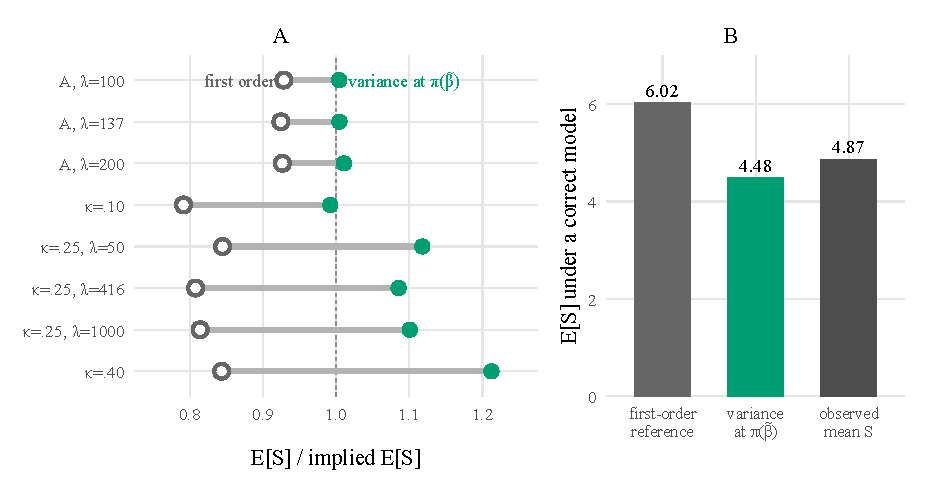
\includegraphics[width=\textwidth]{fig1_mechanism.pdf}
\caption{The fitted-variance deflation. A: the deflation ratio $\delta$ of
(\ref{eq:deflation}) falls short of one in all eight cells under the first-order reference (open
circles), and the shortfall is removed by evaluating the variance at the debiased fit (filled
circles). B: the three quantities at $\kappa = 0.25$, $\lambda = 416$.}
\label{fig:mechanism}
\figalttext[Dumbbell plot of deflation ratios and a three-bar chart]{Panel A shows, for eight
simulation cells, the deflation ratio under the first-order reference at about 0.8 to 0.93 and
under the debiased-variance reference at about 1.0, with the two connected by a grey bar. Panel B
shows three bars: first-order implied mean 6.02, debiased-variance implied mean 4.48, and the
observed mean 4.87.}
\end{figure}

\subsection{The variance at the debiased fit}\label{sec:R2}

Theorem~\ref{thm:variance} suggests the obvious repair: replace $W$ by an estimate of $W_0$. The
natural one is $\widetilde W = \mathrm{diag}\{\tilde\pi_i(1-\tilde\pi_i)\}$ with
$\tilde\pi_i = \pi_i(\bbt)$, the Bernoulli variance at the debiased fit, and the reference
\begin{equation}\label{eq:R2}
  \Sigma_{\mathrm{d}} = A^{\ast}\widetilde WA^{\ast\top}.
\end{equation}
This is exactly the choice the prepivoting bootstrap makes implicitly, since it generates
resampled responses from $\bpi(\bbt)$. Table~\ref{tab:sizeA} reports the consequence. At fixed $p$ $\delta$ moves from $0.93$ to $1.00$--$1.01$ and the size from $0.02$--$0.03$ to
$0.04$--$0.05$; at $\kappa = 0.10$ from $0.79$ to $0.99$ and $0.006$ to $0.054$. Wherever the
first-order theory applies, replacing the variance is the whole correction.

At $\kappa \ge 0.25$, however, (\ref{eq:R2}) over-corrects: $\delta$ rises above one and the size to $0.07$--$0.13$, most where the penalty is lightest. The reason is that $\bbt$ is
now a noisy estimate --- at $\kappa = 0.25$ its correlation with the true index is about $0.7$ ---
so $\tilde\pi_i$ is \emph{more} extreme than $\pi_i$ and $\widetilde W$ understates the null
variance. Two things are needed in the proportional regime: a variance estimate that does not
inherit the noise of $\bbt$, and an account of a second term that the proportional regime
introduces. The next section supplies both.

% =====================================================================
\section{An observable reference in the proportional regime}\label{sec:prop}
% =====================================================================

\subsection{Observable adjustments}\label{sec:bellec}

\citet{bellec2022} studies regularised M-estimators $\bbh = \arg\min_{\boldsymbol{b}}
n^{-1}\sum_i \ell_{y_i}(\bx_i^{\top}\boldsymbol{b}) + g(\boldsymbol{b})$ in single-index models
$y_i = \mathcal{F}(\bx_i^{\top}\boldsymbol{w}, \varepsilon_i)$ with Gaussian design, in the regime where
$p/n$ is bounded, and shows that the mean-field description of $\bbh$ and of the fitted values
$X\bbh$ obtained by \citet{sur2019}, \citet{salehi2019} and others can be expressed through
quantities computed from the data alone. We need three of them, written in our notation. Let
$\bpsi = \by - \hat\bpi$ be the raw residual, let $\hat{\mathrm{df}} = \tr(XM^{-1}X^{\top}W)$,
let $\Gamma = W - WXM^{-1}X^{\top}W$ and $\hat\gamma = \hat{\mathrm{df}}/\tr(\Gamma)$; and let
$\hat a^{2}$ and $\hat\sigma^{2}$ be the estimators of Bellec's equation~(3.20) of, respectively,
the squared inner product of $\bbh$ with the index direction and the squared norm of its
component orthogonal to the index. Then Theorem~4.3 of \citet{bellec2022} gives, for the logistic
loss and each observation,
\begin{equation}\label{eq:bellec}
  \bx_i^{\top}\bbh - \hat\gamma\psi_i \;\approx\; a_{\ast}U_i + \sigma_{\ast}Z_i,
\end{equation}
where $U_i = \bx_i^{\top}\boldsymbol{w}$ is the true index standardised to unit variance,
$Z_i$ is standard normal and independent of $U_i$, and $(a_{\ast}, \sigma_{\ast})$ are
consistently estimated by $(\hat a, \hat\sigma)$ (his Theorem~4.4). Equation~(\ref{eq:bellec}) says that an observable quantity, $m_i = \bx_i^{\top}\bbh - \hat\gamma\psi_i$, equals the true index up to scale plus independent Gaussian noise of known variance. Two points of implementation must be stated. Bellec's model has no intercept and his penalty is strongly convex in every direction, while ours leaves the intercept unpenalised; we centre the design and the fitted index before applying (\ref{eq:bellec}) and refit the intercept in (\ref{eq:w0}) below. And his estimator of $\hat a^{2}$ involves $\Sigma_x^{-1/2}$ with $\Sigma_x$ known; we replace $\Sigma_x$ by the sample covariance of the centred design, a plug-in whose error at
$p/n$ up to $0.4$ is not covered by his Theorem 4.4. Its size can be measured, since in a
simulation the true $\Sigma_x$ is known: over $200$ replications the plug-in raises $\hat\rho$ from
the oracle value by $0.030$ at $\kappa = 0.25$, $0.042$ at $\kappa = 0.40$ and $0.034$ in the
design with weak covariate correlation. The bias is small but it is one-sided, and it is in the
direction that makes the rule of Corollary~\ref{cor:adaptive} keep the cubic direction slightly too
often, which the threshold $\tau$ has to absorb.

\subsection{The de-noised null variance}\label{sec:R5}

Given (\ref{eq:bellec}) and a Gaussian design, the conditional law of the true index given the
fit is Gaussian:
\begin{equation}\label{eq:cond}
  a_{\ast}U_i \mid m_i \;\sim\; \mathcal{N}\!\Bigl(\frac{\hat a^{2}}{\hat a^{2}+\hat\sigma^{2}}\,m_i,\;
  \frac{\hat a^{2}\hat\sigma^{2}}{\hat a^{2}+\hat\sigma^{2}}\Bigr).
\end{equation}
The true linear predictor is $\eta_{0i} = \alpha + c\,a_{\ast}U_i$ for an intercept $\alpha$ and
a scale $c$ that the single-index model leaves free but the known logistic link identifies. We
estimate $(\alpha, c)$ by maximising the marginal likelihood of $\by$ given the conditional law
(\ref{eq:cond}), a one-dimensional integral per observation evaluated by twenty-point
Gauss--Hermite quadrature, and define
\begin{equation}\label{eq:w0}
  \hat w_{0i} = \mathbb{E}\bigl\{\expit(\hat\alpha + \hat c\,\zeta)\,[1 - \expit(\hat\alpha +
  \hat c\,\zeta)] \;\big|\; m_i\bigr\}, \qquad \text{where $\zeta$ has the conditional law (\ref{eq:cond}),}
\end{equation}
the de-noised estimate of the null Bernoulli variance, with $\widehat W_0 =
\mathrm{diag}(\hat w_{0i})$ and the reference $\Sigma_{\mathrm{dn}} = A^{\ast}\widehat W_0A^{\ast\top}$.

\begin{assumption}\label{ass:bellec}
(a) The design has independent rows $\bx_i \sim \mathcal{N}(\boldsymbol{0}, \Sigma_x)$ with the
condition number of $\Sigma_x$ bounded. (b) $p/n$ is bounded above and, for the rates quoted from
\citet{bellec2022}, bounded away from zero, the fixed-dimension case being covered instead by
Theorem~\ref{thm:variance}. (c) The penalty satisfies Assumptions~A and~B of \citet{bellec2022}
after the intercept is removed by centring. (d) The rows of $A^{\ast}$ have entries of order
$n^{-1/2}$, as they do when each group receives a fixed positive proportion of the observations, as
in Assumption~\ref{ass:firstorder}. (e) The logistic scale $c$ is identified and its
maximum-likelihood estimate consistent.
\end{assumption}

Conditions (a) to (c) are those of \citet{bellec2022}, and the ridge penalty of
Section~\ref{sec:notation} meets (c) once the intercept is removed by centring, the remaining
penalty being strongly convex. Condition (d) is the proportional-regime counterpart of the fixed
grouping of Assumption~\ref{ass:firstorder}. Condition (e) is the one that is assumed rather than
shown, and the discussion after the proof reports where the estimate it concerns is good and where
it is not. Assumption~\ref{ass:bellec} binds under the null only: it enters the reference
distribution and therefore governs the size of the test, while under a departure it affects nothing
but the degree that the rule of Corollary~\ref{cor:adaptive} selects, which is why that rule carries
the two guards of Section~\ref{sec:adaptive}.

\begin{proposition}\label{prop:denoised}
Under Assumption~\ref{ass:bellec} and a correctly specified logistic model,
$n^{-1}\sum_i |\hat w_{0i} - \mathbb{E}\{\pi_i(1-\pi_i) \mid m_i\}| \to 0$ in probability, and
hence $\Sigma_{\mathrm{dn}} - A^{\ast}\overline W_0A^{\ast\top} \to 0$, where $\overline W_0 =
\mathrm{diag}[\mathbb{E}\{\pi_i(1-\pi_i)\mid m_i\}]$ is the conditional null variance given the fit.
\end{proposition}

\begin{proof}
By Theorems~4.3 and~4.4 of \citet{bellec2022}, $(\hat\gamma, \hat a^{2}, \hat\sigma^{2})$ converge to
$(\gamma_{\ast}, a_{\ast}^{2}, \sigma_{\ast}^{2})$ and the representation (\ref{eq:bellec}) holds
with an averaged Wasserstein error of order $n^{-1/2}$. With a Gaussian design, (\ref{eq:cond}) is
the exact conditional law of $a_{\ast}U_i$ given $m_i$ under the limiting representation, so the
right-hand side of (\ref{eq:w0}), a bounded Lipschitz functional of $(m_i, \hat a, \hat\sigma,
\hat\alpha, \hat c)$, converges to $\mathbb{E}\{\pi_i(1-\pi_i)\mid m_i\}$ by the continuous-mapping
theorem once $(\hat\alpha, \hat c)$ are consistent, which is the last part of the assumption. The
statement about $\Sigma_{\mathrm{dn}}$ follows from the row-norm condition in Assumption~\ref{ass:bellec}:
writing $\boldsymbol{a}_g$ for the $g$th row of $A^{\ast}$ and $d_i = \hat w_{0i} -
\mathbb{E}\{\pi_i(1-\pi_i) \mid m_i\}$, the $(g,h)$ entry of $A^{\ast}\mathrm{diag}(d)A^{\ast\top}$
is bounded by $\max_g \|\boldsymbol{a}_g\|_{\infty}^{2} \sum_i |d_i|$, which is $O(n^{-1}\sum_i |d_i|)$ by condition~(d) of Assumption~\ref{ass:bellec}, and the first
part of the proposition bounds $n^{-1}\sum_i|d_i|$.
\end{proof}

Three remarks on the proposition. It is stated for the conditional variance given the fit, and its
target is that conditional variance under the limiting representation (\ref{eq:bellec}) rather than the exact finite-sample conditional variance; the two differ by the Wasserstein error of Bellec's theorem. And its last hypothesis is not proved here: the scale $c$ enters only through the known link, and consistency of its one-dimensional maximum-likelihood estimate is what one expects but is stated as an assumption so that the reader knows where the proof stops. Estimating the signal strength of a high-dimensional logistic model from data alone is a solved problem for the maximum likelihood estimator, by the ProbeFrontier method of \citet{sur2019} and by SLOE \citep{yadlowsky2021}; those estimators are built for the maximum likelihood fit and do not apply to a ridge fit at a penalty of the analyst's choosing, which is why the scale is estimated here from the conditional law (\ref{eq:cond}). The estimate is constrained to $c \in [0.05, 20]$, a box introduced after an unconstrained search
diverged on a small number of replications. Finally, the covariance Theorem~\ref{thm:variance} calls
for is $A^{\ast}W_0A^{\ast\top}$, while the proposition delivers
$A^{\ast}\overline W_0A^{\ast\top}$. Their difference has $(g,h)$ entry
$\sum_i a_{gi}a_{hi}d_i$ with $d_i = \pi_i(1-\pi_i) - \mathbb{E}\{\pi_i(1-\pi_i) \mid m_i\}$
conditionally centred and bounded by $1/4$, and weights of order $n^{-1}$ by condition~(d); the sum
is $o_p(1)$ provided the $d_i$ are weakly dependent, which we assume. Empirically the estimate is good where the penalty is moderate and poor where it is light. Across the twenty-five designs of Section~\ref{sec:sim}, whose proportional-regime cells are
design~B$'$ and so have a true standard deviation of the linear predictor of $2.31$, it recovers
that standard deviation within 3 per cent at fixed $p$ and within 16 per cent in seventeen of the
eighteen proportional-regime cells at $\lambda \ge 416$, under Gaussian, heavy-tailed and binary
predictors alike, the exception being the heaviest penalty at the largest aspect ratio,
$\kappa = 0.40$, $\lambda = 1000$, where it understates the scale by 24 per cent; at the
lightest penalties it overstates the scale badly, by 21 per cent at $\kappa = 0.25$, $\lambda = 50$
and by 58 per cent at $\kappa = 0.40$, $\lambda = 50$. Those are also the cells in which the decile
statistic is least reliable, and the two facts are connected: an overstated scale understates the
null variance.

Table~\ref{tab:sizeA} shows what the de-noised variance buys. It coincides with (\ref{eq:R2}) at
fixed $p$, repairs the cell in which $\bbt$ overshoots most ($\kappa = 0.25$, $\lambda = 50$:
size $0.046$ against $0.086$), and halves the excess at $\kappa = 0.40$. A residual of one to
three percentage points remains at $\kappa \ge 0.25$, and it is not a variance.

\subsection{The selection non-centrality}\label{sec:selection}

The remaining term is a mean. Under a correct model the corrected residual should average zero in
every group; at $\kappa = 0.25$ it does not. Over 300 replications of design~B at $\lambda = 416$
the squared norm of the mean of $\bv$ is $0.288$ ($300$ replications; the Monte Carlo floor, the value expected from sampling error alone, is
$\tr(\Om_{\mathrm{MLE}})/300 \approx 0.020$), and its
shape across the ten groups is the S-curve of Figure~\ref{fig:selection}A. Holding the grouping
fixed --- forming the deciles from the fitted index of the noise-free response
$\bpi(\bb)$, a function of $X$ alone --- reduces it to $0.077$, with the deflation ratio
unchanged. Most of the term is therefore created by grouping on the fitted index. The remainder is
not: $0.077$ is about six times the Monte Carlo floor, and it is the second-order part of the
shrinkage displacement, which the plug-in $\hat\bmu$ removes only to first order. A delta-method
expansion of $\hat\bmu$ about $\bbt$ predicts $0.067$ for it, close to what is observed, and its
effect on the size of the test is at most $0.007$ in this cell.

The mechanism is regression to the mean, and we call it response-dependent grouping. The fitted
index is a noisy version of the true one, and
an observation reaches the top decile partly because its own noise was positive; noise is
positive when $y_i$ exceeded its expectation, so the top decile is enriched with events beyond
what its probabilities justify, and the bottom decile depleted. That argument gives the existence
and the order of the term in the raw grouped residual; in the corrected residual $\hat\bmu$ absorbs
most of it, and the cubic shape of what survives is an empirical finding rather than a consequence
of the argument. At fixed $p$ the self-influence of $y_i$ on $\hat\eta_i$ \citep{pregibon1981} is $h_{ii} = w_i\bx_i^{\top}M^{-1}\bx_i$, of order $p/n$, and the effect is
negligible; in the proportional regime it is of order $\kappa$. This is the random-cells effect of \citet{moore1975}, which is $o(1)$ in their setting and $O(1)$
here. The groups are formed in part from the responses they are then used to test.

\begin{elaw}\label{lem:order}
Let $\bar h = \hat{\mathrm{df}}/n$ be the mean self-influence. Across the eight cells of
Section~\ref{sec:sim}, the fraction $\hat g = \|\mathbb{E}\bv\|^{2}/\tr(\Om_{\mathrm{MLE}})$ satisfies
$\hat g \approx 0.24\,\kappa$ (coefficient of determination $0.93$), and equivalently
$\hat g \approx 0.28\,\bar h^{1/2}$; restricted to the three-dimensional EDGE subspace, and
normalised there by the trace the reference itself supplies on that subspace,
$\hat g_{\mathrm E} = \|P_Z\mathbb{E}\bv\|^{2}/\tr(P_Z\Sigma_{\mathrm{dn}}) \approx 1.15\,\kappa$ ($0.97$), and 90 to 98 per cent of
$\|\mathbb{E}\bv\|^{2}$ lies in that subspace when $\kappa > 0$, almost none of it in the directions of degree at most two.
The constants are fitted on those eight cells and are not derived; the relation is written in
$\kappa$ because $\kappa$ orders the cells examined here, and Section~\ref{sec:heldout} shows that
the quantity the term really tracks is the self-influence measured against the spread of the fitted
index, so the relation should not be carried to design families in which those two move apart. The two
fractions are normalised differently: the decile constant is fitted against the first-order trace
$\tr(\Om_{\mathrm{MLE}})$, which exceeds $\tr(\Sigma_{\mathrm{dn}})$ across these cells, and fitted
against $\tr(\Sigma_{\mathrm{dn}})$ instead it would be $0.30\,\kappa$ ($0.96$). CALM applies
$0.24\,\kappa$, so on the decile basis the inflation is a calibrated factor rather than an exact
mean match.
\end{elaw}

Section~\ref{sec:heldout} reports what happens in cells that were not used to fit the constants.
The content of the relation is in Figure~\ref{fig:selection}B. Two consequences are immediate. First, the non-centrality can
be placed in the distribution by inflating the scale of the reference to
$(1 + \hat g)\Sigma_{\mathrm{dn}}$, and because a scaled central weighted chi-squared with the
correct mean has a heavier upper tail than the true non-central one, an inflation that matches the
mean can only err towards conservatism. On the EDGE subspace it does match, since
$\hat g_{\mathrm E}$ is normalised by the same $\tr(P_Z\Sigma_{\mathrm{dn}})$ that the reference
supplies there. On the decile basis it does not: $\hat g$ is normalised by the larger first-order
trace, so the mean is under-matched and the level that CALM-D holds in Table~\ref{tab:sizeA} is
measured rather than implied. Second, and more
usefully, the term is a cubic. It lives in exactly the direction of the EDGE basis that the
attenuation law says carries no power when the index is noisy.

\begin{figure}[!t]
\centering
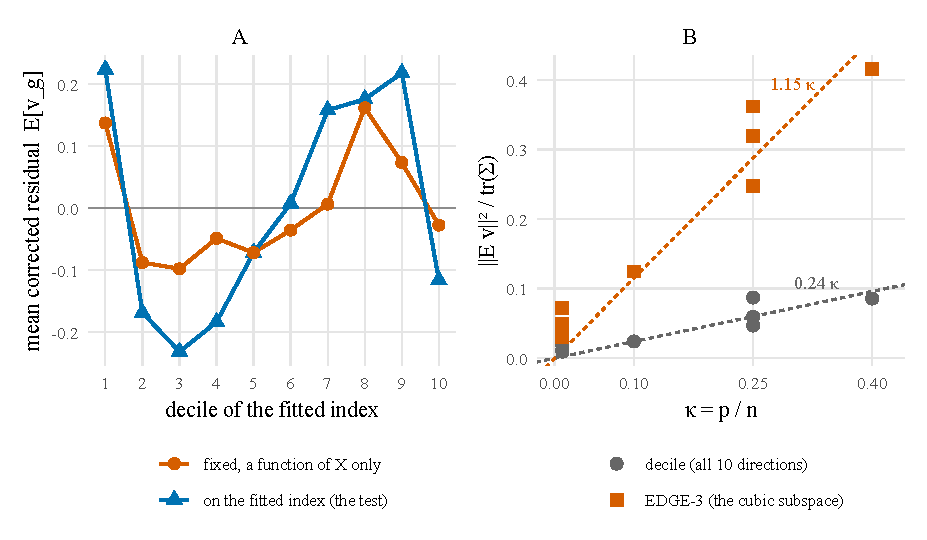
\includegraphics[width=\textwidth]{fig2_selection.pdf}
\caption{The selection non-centrality. A: mean corrected residual by decile at $\kappa = 0.25$,
$\lambda = 416$, when the groups are formed on the fitted index and when they are held fixed as a
function of the design. B: the non-centrality fraction against $\kappa$ for the decile basis and
for the three-dimensional EDGE subspace, with the fitted lines $0.24\kappa$ and $1.15\kappa$.}
\label{fig:selection}
\figalttext[Two panels: an S-shaped curve of group means and a scatter of non-centrality against
kappa with two fitted lines]{Panel A plots the mean corrected residual in each of ten deciles;
with grouping on the fitted index it swings between about minus 0.23 and plus 0.22 in an S-shape,
with fixed grouping it stays within plus or minus 0.16. Panel B plots the non-centrality fraction
against kappa from 0.01 to 0.40 for two bases, with points near the lines 0.24 kappa (decile) and
1.15 kappa (EDGE).}
\end{figure}

\subsection{The adaptive basis}\label{sec:adaptive}

\begin{proposition}[Attenuation law, \citealp{ebrahim2026seriesc}]\label{prop:atten}
Let $\eta^{\ast}$ and $\hat\eta^{\ast}$ be the true and fitted linear predictors, standardised,
jointly Gaussian with correlation $\rho$. A departure equal to the degree-$k$ Hermite component of
the true predictor survives grouping on the fitted predictor with amplitude $\rho^{k}$, and its
non-centrality is attenuated by $\rho^{2k}$.
\end{proposition}

The correlation $\rho$ is not a nuisance one must guess. Under (\ref{eq:bellec}) it is
\begin{equation}\label{eq:rho}
  \hat\rho = \frac{\hat a}{\sqrt{\hat a^{2} + \hat\sigma^{2}}},
\end{equation}
an observable, which we call the index correlation: it is computed from one fit and it measures how
much of the true index survives in the fitted one, so it is the quantity that decides what a grouped
test can see. By Proposition~\ref{prop:atten} a degree-$k$ departure reaches the groups with
$\rho^{2k}$ of its non-centrality, so $\hat\rho$ converts directly into a statement about power: at
$\hat\rho = 0.7$ a quadratic departure retains about a quarter of its non-centrality and a cubic
departure about an eighth. Any diagnostic that groups or bins on a fitted index can compute
$\hat\rho$ from its own fit and read off the same limit. It equals $0.94$ in design~A, $0.71$ at
$\kappa = 0.10$, $0.69$ at $\kappa = 0.25$ and $0.92$ on the glaucoma data. Two approximations are involved in using it. It is the correlation of
the adjusted index $m_i$ with the truth, while the groups are formed on $\hat\eta_i$, which differs
from $m_i$ by the self-influence term of Section~\ref{sec:selection}; and
Proposition~\ref{prop:atten} concerns Hermite components of a continuous predictor, while the EDGE
basis is a set of orthogonal polynomials over $G$ discrete group means, so ``zero otherwise'' in
the corollary holds up to the error of that discretisation. Both approximations improve as $G$
grows and as the self-influence falls.

\begin{corollary}\label{cor:adaptive}
Among EDGE bases of degree $k \le 3$ referred to the same null law, the retained non-centrality of
a degree-$j$ departure is $\rho^{2j}$ if $j \le k$ and zero otherwise, while the basis spends $k$
degrees of freedom. Keeping the cubic direction only when $\hat\rho^{6} \ge \tau$, for a threshold
$\tau \in (0,1)$, therefore retains it exactly when its signal survives at fraction $\tau$. With
$\tau = 0.2$ the rule takes $k = 3$ when $\hat\rho \ge 0.76$ and $k = 2$ otherwise, and we keep the
cubic in addition whenever $\kappa < 0.05$, where there is no selection term to avoid.
\end{corollary}

\begin{proof}
By Proposition~\ref{prop:atten} the degree-$j$ Hermite component of a departure survives grouping
on the fitted predictor with amplitude $\rho^{j}$, so the non-centrality it contributes in the
direction of the degree-$j$ orthogonal polynomial is $\rho^{2j}$. An EDGE basis of degree $k$
contains that direction when $j \le k$ and is orthogonal to it otherwise, up to the discretisation
error noted above, and it spends one degree of freedom on each of its $k$ directions. Keeping the
cubic direction when $\hat\rho^{6} \ge \tau$ therefore keeps it exactly when the fraction
$\rho^{6}$ of the cubic non-centrality that survives grouping is at least $\tau$.
\end{proof}

The value of the corollary is in the second consequence of
Fitted relation~\ref{lem:order}: when the index is noisy the rule drops the cubic direction, which by
Proposition~\ref{prop:atten} retains about $\rho^{6} \approx 0.12$ of any cubic departure and by
Fitted relation~\ref{lem:order} carries almost all of the selection non-centrality. One decision removes a
powerless direction and a biased one. Two guards are needed, and both exist because $\hat\rho$ is a null quantity: under a misspecified
model the representation (\ref{eq:bellec}) reads the misfit as noise and $\hat\rho$ falls, so a rule
that used $\hat\rho$ alone would discard directions precisely when a departure occupies them. The
first guard is the floor at two. A degree-one basis is the calibration-slope direction alone and
cannot see any change of shape, and in the simulations of Section~\ref{sec:power} $\hat\rho$ fell
from $0.66$--$0.71$ under the null to $0.44$--$0.60$ under the strongest departures, which without
a floor would have cost the quadratic direction. The second is the aspect-ratio clause. At fixed
$p$ the selection term is negligible, so there is nothing to gain by dropping the cubic, and
$\hat\rho$ falls from $0.93$ under the null to $0.75$ under a strong cubic departure --- across the
threshold, and therefore into discarding the direction that carries the signal, at a cost of $0.60$
in power (Section~\ref{sec:degree}). Keeping $k = 3$ whenever $\kappa < 0.05$ removes that failure
without affecting any proportional-regime cell. What remains is a single decision, whether to keep
the cubic when the index is noisy, and the rule makes it correctly on the glaucoma data of
Section~\ref{sec:glaucoma}, where $\hat\rho = 0.92$ and the misfit lies in the cubic direction.
Table~\ref{tab:tau} reports the sensitivity to $\tau$: values below $0.2$ keep the cubic too often
and the size rises to $0.61$--$0.86$ in the design where the selection term is largest, while
$\tau = 0.3$ behaves like $\tau = 0.2$ and would still keep the cubic on the glaucoma data, where
$\hat\rho^{6} = 0.61$.

 We call the result the
\emph{adaptive} EDGE basis and write EDGE-$\rho$ where a symbol is needed.

\subsection{Definition of CALM}\label{sec:calm}

CALM refers the shrinkage-corrected statistics of (\ref{eq:stats}) to the exact weighted
chi-squared law of Section~\ref{sec:davies} with covariance $(1 + \hat g)\Sigma_{\mathrm{dn}}$, where
$\Sigma_{\mathrm{dn}}$ is the de-noised reference of Section~\ref{sec:R5}, $\hat g$ is the basis-specific
non-centrality fraction of Fitted relation~\ref{lem:order} ($0.24\kappa$ for the decile basis,
$1.15\kappa$ for EDGE-3 and $0.11\kappa$ for EDGE of degree at most two), and the EDGE basis is
the adaptive one of Corollary~\ref{cor:adaptive} together with the aspect-ratio clause that
follows it. It requires one penalised fit and no resampling. At fixed $p$ the inflation is negligible ($\hat g = 0.002$) and CALM is the reference
(\ref{eq:R2}). Table~\ref{tab:algorithm} states the whole procedure, and names the result that
licenses each step.

\begin{table}[!t]
\centering
\caption{CALM in full. The inputs are one penalised fit and the analyst's own grouping; there is no
resampling, and every step is a closed-form computation on quantities the fit already provides. The
right-hand column names the result that licenses the step.}
\label{tab:algorithm}
\small
\begin{tabular}{p{0.66\textwidth}l}
\toprule
\multicolumn{2}{l}{\emph{Input}: design $X$ with intercept column, responses $\by$, penalty
$\lambda$, number of groups $G$, threshold $\tau = 0.2$.} \\
\midrule
1. Fit the penalised model; form $\bbh$, $\hat\bpi$, $W$, $F$, $K$ and $M$, the $G$
equal-frequency groups of $\hat\bpi$ with $C$ and $V$, and $U$ and $\br$.
  & Section~\ref{sec:notation} \\
2. Debias in one step, $\bbt = \bbh + F^{-1}K\bbh$; form $\bv = \br - UM^{-1}K\bbt$ and
$A^{\ast} = V^{-1/2}C - UF^{-1}X^{\top}$.
  & (\ref{eq:firstorder}) \\
3. Centre the design; form $\bpsi = \by - \hat\bpi$, $\hat\gamma$, $(\hat a, \hat\sigma)$ and
$m_i = \bx_i^{\top}\bbh - \hat\gamma\psi_i$.
  & (\ref{eq:bellec}) \\
4. Estimate $(\hat\alpha, \hat c)$ by maximising the marginal likelihood under (\ref{eq:cond});
form $\hat w_{0i}$ and $\Sigma_{\mathrm{dn}} = A^{\ast}\widehat W_0A^{\ast\top}$.
  & Proposition~\ref{prop:denoised} \\
5. Compute the index correlation $\hat\rho$ and take $k = 3$ if $\hat\rho^{6} \ge \tau$ or
$\kappa < 0.05$, and $k = 2$ otherwise; the decile basis instead spends all $G$ directions.
  & Corollary~\ref{cor:adaptive} \\
6. Inflate the reference to $(1 + \hat g)\Sigma_{\mathrm{dn}}$, with $\hat g = 0.24\kappa$ on the
decile basis, $1.15\kappa$ on EDGE-3 and $0.11\kappa$ on EDGE of degree at most two.
  & Fitted relation~\ref{lem:order} \\
7. Refer SC.HL or SC.EDGE to the weighted chi-squared law with that covariance, evaluated by the
algorithm of \citet{davies1980}.
  & Section~\ref{sec:davies} \\
\midrule
\multicolumn{2}{l}{\emph{Output}: the $p$-value for $H_0^{\mathrm{str}}$ along the fitted index, and
the degree $k$ that step~5 selected.} \\
\bottomrule
\end{tabular}
\end{table}


An implementation of Table~\ref{tab:algorithm} as a single function, \texttt{calm.gof()}, is in
the reproduction archive \citep{ebrahim2026calm}.

We write CALM-E for the test on the adaptive EDGE basis and CALM-D for the test on the decile
basis, and use those names wherever the two differ.

The two bases are not on the same footing in the proportional regime, and Section~\ref{sec:heldout} shows why this matters. The adaptive EDGE basis removes the selection term by dropping the direction that carries it, so
the inflation is inert there while the rule takes degree two, as it does in every
proportional-regime cell here: the factor is then at most $1.05$, and removing it altogether changes
the size by at most $0.008$ in every cell we examined (Section~\ref{sec:sim}). We keep it in the
definition for uniformity across bases, and the statistic would behave the same without it. The decile basis spends all $G$ directions, so it cannot avoid that direction and must instead absorb it into the reference through $\hat g$, a quantity that was fitted on eight cells. We therefore recommend the adaptive EDGE basis as the primary statistic and report the decile
statistic, which is the shrinkage-corrected Hosmer--Lemeshow test and the one a reader of that
tradition will look for, alongside it. The recommendation is not a preference between two equally
good options. It is the one design in which holding the level does not depend on a constant fitted to reproduce
the selection term, and Section~\ref{sec:heldout} shows that this is what survives designs the
constants never saw. It is not free of tuning: the degree rule carries the threshold $\tau$, whose
value is fixed in Section~\ref{sec:adaptive} and whose influence on the size is reported in
Table~\ref{tab:tau}.

% =====================================================================
\section{Numerical results}\label{sec:sim}
% =====================================================================

\subsection{Designs}\label{sec:designs}

We use the registered designs of \citet{ebrahim2026seriesc} so that every number can be
compared with that paper. Design~A has $n = 500$, $p = 5$, independent standard normal covariates,
$\bb = (0.5,-0.4,0.3,-0.3,0.2)^{\top}$ and $\lambda \in \{100, 137, 200\}$. Design~B has
$n = 400$, an autoregressive covariate correlation of $0.7$, coefficients cycling
$(0.35,-0.30,0.25,-0.20,0.15)$ scaled to $\|\bb\| = 2.31$, and $p = 100$ ($\kappa = 0.25$) with
$\lambda \in \{50, 416, 1000\}$; a $\kappa$ sweep keeps $\lambda = 416$ and takes $p = 40$ ($\kappa = 0.10$) and $p = 160$
($\kappa = 0.40$). Under that scaling the standard deviation of the linear predictor is $1.48$ to
$1.51$ across the three dimensions. A second scaling of the same coefficients is used from
Table~\ref{tab:heldout} onwards and we write design~B$'$ for it: there the coefficients are scaled so
that the standard deviation of the linear predictor, rather than $\|\bb\|$, equals $2.31$, which
makes $\|\bb\|$ equal to $3.54$ to $3.61$ and the signal about half again as strong. The two are not
interchangeable, and we say which is used wherever it matters: Table~\ref{tab:sizeA},
Tables~\ref{tab:power}, \ref{tab:invalid} and \ref{tab:boundary},
Figure~\ref{fig:attenuation} and the supplementary material report design~B, and the constants of
Fitted relation~\ref{lem:order} were fitted there; Tables~\ref{tab:heldout}, \ref{tab:tau},
\ref{tab:decomp} and \ref{tab:gaps}, and the scale-recovery figures of Section~\ref{sec:R5}, report
design~B$'$. All fits are ridge logistic regression by
penalised iteratively reweighted least squares with the intercept unpenalised; $G = 10$ throughout.
Under the null, data are generated from the design's own model, so every rejection is a false
one. Sizes are based on 500 replications unless stated, for a Monte Carlo standard error of $0.010$ at
the $5$ per cent level. Code that reproduces every number, table and figure below, with the random
seeds, is in the reproduction archive \citep{ebrahim2026calm}.

\subsection{Size}

\begin{table}[!t]
\centering
\caption{Rejection rate of a correctly specified model at nominal level $0.05$ under four
references, eight cells: the first-order reference is conservative everywhere, the variance at the
debiased fit is liberal at $\kappa \ge 0.25$, the de-noised variance repairs the lightest-penalty
cell, and CALM holds the level on the decile basis and is conservative on the EDGE basis in the
proportional regime. The first three EDGE columns use EDGE-3; the CALM columns use the adaptive EDGE
basis and the basis-specific inflation of Section~\ref{sec:calm}. $500$ replications per cell.}
\label{tab:sizeA}
\small
\begin{tabular}{llcccccccc}
\toprule
& & \multicolumn{4}{c}{Decile basis (SC.HL)} & \multicolumn{4}{c}{EDGE basis (SC.EDGE)} \\
\cmidrule(lr){3-6}\cmidrule(lr){7-10}
Design & $\lambda$ & first order & $\Sigma_{\mathrm d}$ & $\Sigma_{\mathrm{dn}}$ & CALM-D & first order & $\Sigma_{\mathrm d}$ & $\Sigma_{\mathrm{dn}}$ & CALM-E \\
\midrule
A ($\kappa = 0.01$) & 100  & 0.030 & 0.044 & 0.046 & 0.046 & 0.028 & 0.050 & 0.048 & 0.050 \\
A                   & 137  & 0.022 & 0.036 & 0.040 & 0.038 & 0.030 & 0.040 & 0.038 & 0.040 \\
A                   & 200  & 0.018 & 0.044 & 0.046 & 0.046 & 0.030 & 0.050 & 0.048 & 0.048 \\
\addlinespace
B, $\kappa = 0.10$  & 416  & 0.006 & 0.054 & 0.066 & 0.060 & 0.012 & 0.048 & 0.054 & 0.040 \\
B, $\kappa = 0.25$  & 50   & 0.020 & 0.086 & 0.046 & 0.032 & 0.030 & 0.120 & 0.056 & 0.006 \\
B, $\kappa = 0.25$  & 416  & 0.018 & 0.076 & 0.072 & 0.052 & 0.024 & 0.080 & 0.076 & 0.028 \\
B, $\kappa = 0.25$  & 1000 & 0.014 & 0.072 & 0.052 & 0.036 & 0.034 & 0.082 & 0.072 & 0.030 \\
B, $\kappa = 0.40$  & 416  & 0.022 & 0.128 & 0.054 & 0.036 & 0.036 & 0.108 & 0.084 & 0.018 \\
\bottomrule
\end{tabular}
\end{table}

Table~\ref{tab:sizeA} gives the size of the four references. The
first-order reference is conservative everywhere and severely so at $\kappa = 0.10$, where it
rejects $0.6$ per cent of correct models. The variance at the debiased fit holds its level at fixed $p$
and at $\kappa = 0.10$ and is liberal at $\kappa \ge 0.25$. The de-noised variance repairs the
lightest-penalty cell and halves the excess at $\kappa = 0.40$. CALM holds the level on the decile basis, where every cell is within Monte Carlo error of the
nominal level, and never exceeds it on the EDGE basis: there the rule of
Corollary~\ref{cor:adaptive} drops the cubic direction in the proportional regime, and the
two-dimensional basis rejects $0.6$ to $4$ per cent of correct models, least at $\kappa = 0.25$,
$\lambda = 50$. That conservatism is not caused by the inflation, and it is not an artefact of the level: Section~S3 of the supplementary material repeats the check at $0.01$ and $0.10$, where the adaptive statistic rejects between $0.000$ and $0.062$ and between $0.030$ and $0.154$ of correct models. On the EDGE basis the factor is at most $1.05$
while the rule takes degree two, as it does in every proportional-regime cell here,
and removing it altogether changes the size by at most $0.008$ in every cell we examined; the
de-noised reference overstates the null variance in the low-degree directions while understating it
in the cubic direction, and dropping the cubic leaves only the overstated part. We keep the
inflation on this basis for consistency of definition rather than for its effect, and the statistic
would behave the same without it.

\subsection{Robustness to the design law}\label{sec:designlaw}

Assumption~\ref{ass:bellec} requires Gaussian predictors. Table~S2 of the supplementary material
repeats three cells with predictors drawn from a $t_3$ distribution scaled to unit variance and from
a standardised Bernoulli$(0.3)$ law, and finds the size of the de-noised reference between $0.042$ and $0.098$, the worst being the
heavy-tailed design, where the level doubles. Gaussianity is a condition of the proof rather than a
hard boundary of the method, but the heavy-tailed cells are consistently the least reliable. Section~\ref{sec:heldout} goes further and runs the whole procedure under those two laws.

\subsection{Validation outside the calibration cells}\label{sec:heldout}

The constants of Fitted relation~\ref{lem:order} were fitted on the eight cells of
Table~\ref{tab:sizeA}, and Table~\ref{tab:sizeA} therefore reports the size of CALM in the cells
that calibrated it. Table~\ref{tab:heldout} reports it in seventeen further cells: two
intermediate aspect ratios, two penalties at $\kappa = 0.40$, a design with covariate correlation
$0.3$ instead of $0.7$, a weaker and a stronger signal than design~B$'$, a design twice the size at
the same aspect ratio, twenty groups instead of ten, and the three predictor laws of
Section~\ref{sec:designlaw} run through the whole procedure rather than through
$\Sigma_{\mathrm{dn}}$ alone. Sixteen of the seventeen did not calibrate the constants; the
exception is the $\mathrm{sd}(\eta) = 1.5$ row, which is design~B at $\lambda = 416$ up to the
scaling, and which we report at an independent seed as a check on Monte Carlo error rather than as a
held-out cell.

The two bases behave differently, and the difference is the main practical finding of this
section. On the adaptive EDGE basis the size lies between $0.024$ and $0.080$ in every one of the
seventeen cells, with fifteen of them within three Monte Carlo standard errors of the
nominal level and the largest at $0.080$; the level there does not rest on a constant fitted to the selection term, because the rule of
Corollary~\ref{cor:adaptive} drops the direction that term occupies rather than
correcting for it. On the decile basis, which spends all $G$ directions and must therefore absorb
that term into the reference through $\hat g$, the size is between $0.034$ and $0.076$ in twelve
cells and fails in the remaining five, most severely at covariate correlation $0.3$, where it
rejects $0.688$ of correct models.

\textbf{Where the decile correction fails, and why.} The failures have one cause, and it is visible
in Fitted relation~\ref{lem:order} itself: the selection term is not a function of $\kappa$. An observation changes group when its own response
moves its fitted index across a group boundary, so the term grows with the self-influence
$\bar h$ measured against the spread of the fitted index, and with the number of observations per
group. At $\kappa = 0.25$ the squared mean $\|\mathbb{E}\bv\|^{2}$ is nine times larger under
covariate correlation $0.3$ than under $0.7$, because the fitted index has half the spread there
while the self-influence is unchanged, and it doubles when $n$ doubles at fixed $\kappa$. The quantity
\begin{equation}\label{eq:crossing}
  \hat q = n\bar h^{2}/\mathrm{sd}(\hat\eta)^{2},
\end{equation}
which the boundary-crossing argument suggests and which we call the crossing index, tracks the term
across these designs better than $\kappa$ does but not closely enough to replace it, and a
per-dataset estimate built from the leave-one-out displacement of the index proved far too noisy to
use. The open problem is therefore precise: is there an observable, built from the self-influence
and the spread of the fitted index, that predicts $\|\mathbb{E}\bv\|^{2}$ well enough to replace the
constant $0.24\kappa$ across design families? Until there is, the decile reference should be read as
calibrated for designs resembling those of Table~\ref{tab:sizeA}. The prepivoting bootstrap is not a way out:
in the two failing designs we also ran it, its size is $0.11$ and $0.07$, so the difficulty is in the corrected statistic and not in the analytic reference alone. The
obstruction is therefore a property of grouping on a noisy index, not of the reference proposed
here, and the comparison of the two bases is itself the finding: a statistic that spends every
direction has to model the selection term, while a statistic that chooses its directions can avoid
it. Where a diagnostic has that freedom, avoiding the contaminated direction proved more robust than
correcting for it wherever that direction stays put, which under balanced outcomes it does, because
the correction needs a constant fitted on particular designs and the avoidance needs none;
Section~\ref{sec:gaps} reports the regime in which the direction moves and the ordering of the two
bases reverses. We record the transfer of that correction as the outstanding problem for
anyone who wants the test in its Hosmer--Lemeshow form rather than its smooth one.

\begin{table}[!t]
\centering
\small
\caption{Rejection rate of a correctly specified model at nominal level $0.05$ in designs that were not used to calibrate the constants of Fitted relation~\ref{lem:order}: nine designs with the Gaussian predictor law and eight repetitions of earlier cells under $t_3$ and standardised Bernoulli predictors. The last column is the mean of the observable $\hat\rho$. $500$ replications per cell; the Monte Carlo standard error is $0.010$. Design~B$'$ of Section~\ref{sec:designs} throughout.}
\label{tab:heldout}
\begin{tabular}{lcccc}
\toprule
Design & CALM-D & CALM-E & EDGE-3 & $\hat\rho$ \\
\midrule
\multicolumn{5}{l}{\emph{New designs, Gaussian predictors}} \\
$\kappa = 0.15$ ($p = 60$) & 0.066 & 0.054 & 0.080 & 0.73 \\
$\kappa = 0.33$ ($p = 132$) & 0.052 & 0.030 & 0.060 & 0.72 \\
$\kappa = 0.40$, $\lambda = 50$ & 0.130 & 0.024 & 0.138 & 0.70 \\
$\kappa = 0.40$, $\lambda = 1000$ & 0.034 & 0.056 & 0.062 & 0.73 \\
$\kappa = 0.25$, correlation $0.3$ & 0.688 & 0.076 & 0.872 & 0.70 \\
$\kappa = 0.25$, $\mathrm{sd}(\eta) = 1.5$ & 0.054 & 0.028 & 0.030 & 0.69 \\
$\kappa = 0.25$, $\mathrm{sd}(\eta) = 3.0$ & 0.082 & 0.080 & 0.132 & 0.74 \\
$\kappa = 0.25$, $n = 800$, $p = 200$ & 0.122 & 0.074 & 0.168 & 0.74 \\
$\kappa = 0.25$, $G = 20$ & 0.044 & 0.056 & 0.102 & 0.73 \\
\addlinespace
\multicolumn{5}{l}{\emph{Other predictor laws}} \\
A, $t_3$ & 0.050 & 0.050 & 0.050 & 0.92 \\
A, binary & 0.052 & 0.058 & 0.058 & 0.94 \\
$\kappa = 0.10$, $t_3$ & 0.112 & 0.080 & 0.164 & 0.72 \\
$\kappa = 0.10$, binary & 0.064 & 0.074 & 0.094 & 0.73 \\
$\kappa = 0.25$, $t_3$ & 0.066 & 0.044 & 0.084 & 0.72 \\
$\kappa = 0.25$, binary & 0.054 & 0.044 & 0.072 & 0.72 \\
$\kappa = 0.40$, $t_3$ & 0.076 & 0.050 & 0.094 & 0.71 \\
$\kappa = 0.40$, binary & 0.056 & 0.044 & 0.078 & 0.72 \\
\bottomrule
\end{tabular}
\end{table}

\begin{table}[!t]
\centering
\small
\caption{Sensitivity of the size of the adaptive EDGE statistic to the threshold $\tau$ of Corollary~\ref{cor:adaptive}, at nominal level $0.05$, in seven designs. The value used throughout is $\tau = 0.2$. $500$ replications per cell; the
$\tau = 0.2$ column is an independent run from the one behind the CALM-E column of
Table~\ref{tab:sizeA}, and the two differ by one to two Monte Carlo standard errors. Design~B$'$ of Section~\ref{sec:designs} throughout.}
\label{tab:tau}
\begin{tabular}{lcccc}
\toprule
& \multicolumn{4}{c}{threshold $\tau$} \\
\cmidrule(lr){2-5}
Design & 0.05 & 0.10 & 0.20 & 0.30 \\
\midrule
A ($\kappa = 0.01$) & 0.050 & 0.050 & 0.050 & 0.050 \\
B, $\kappa = 0.10$ & 0.070 & 0.070 & 0.052 & 0.040 \\
B, $\kappa = 0.25$ & 0.062 & 0.064 & 0.044 & 0.032 \\
B, $\kappa = 0.40$ & 0.048 & 0.040 & 0.032 & 0.024 \\
$\kappa = 0.40$, $\lambda = 50$ & 0.138 & 0.092 & 0.024 & 0.022 \\
$\kappa = 0.25$, correlation $0.3$ & 0.856 & 0.610 & 0.076 & 0.024 \\
$\kappa = 0.10$, $t_3$ & 0.162 & 0.156 & 0.080 & 0.048 \\
\bottomrule
\end{tabular}
\end{table}

\subsection{Unbalanced outcomes, smaller samples and other groupings}\label{sec:gaps}

Three design families lie wholly or partly outside Table~\ref{tab:heldout} and a reader of the clinical prediction
literature will ask about all three. Table~\ref{tab:gaps} reports them, and the first is a boundary
of the method rather than a further confirmation of it.

Outcomes here have been balanced. Shifting the intercept breaks both statistics in the proportional
regime: at $\kappa = 0.25$ the decile statistic rejects $0.060$, $0.204$ and $0.492$ of correct models at
prevalences $0.30$, $0.15$ and $0.08$, and the smooth statistic $0.140$, $0.574$ and $0.884$: the
smooth statistic loses its level first, already at a prevalence of $0.30$. At fixed dimension the decile statistic is unaffected, at $0.054$ and
$0.050$, but the smooth one is not: its size rises to $0.088$ at prevalence $0.15$ and to $0.130$ at
prevalence $0.08$, eight Monte Carlo standard errors above the nominal level, so the loss there is
much smaller than in the proportional regime without being absent. The order is the reverse of the balanced case, where the smooth basis
was the reliable one. The cause is the selection term of Section~\ref{sec:selection}, and it can be
isolated. Let the ratio $\mathbb{E}(S) / \mathbb{E}\{\tr(P_Z \Sigma_{\mathrm{dn}})\}$, on the adaptive EDGE
basis and with $\Sigma_{\mathrm{dn}}$ un-inflated, be the quantity the reference has to reproduce, equal to one when the reference is correct, and split it into the part
contributed by the selection mean $\boldsymbol{m} = \mathbb{E}(\bv)$ and a remainder.
Table~\ref{tab:decomp} reports the split. The remainder stays between $0.88$ and $1.00$ as the
prevalence falls from $0.50$ to $0.08$, so the de-noised variance of Section~\ref{sec:R5} remains
accurate throughout, including where $\hat\rho$ has fallen to $0.62$; the entire excess is
non-centrality, whose share grows from $0.24$ to $8.91$ against the inflation of $0.03$ that the
$\kappa$-law supplies.

Two properties of the selection mean move together, and between them they say why the smooth basis
fares worse. Its squared length grows from $0.59$ to $5.05$. Its shape also turns. Under balanced
outcomes the displacement is the odd, cubic curve that the self-influence argument predicts, and the
quadratic basis retains two per cent of it, which is precisely why the degree rule of
Section~\ref{sec:adaptive} discards the cubic in the proportional regime and why the inflation
constant at degree two is a tenth of the one at degree three; at prevalence $0.08$ the displacement
is a U-shape and the quadratic basis retains ninety-nine per cent. The rule is calibrated on the
premise that the term to be avoided is cubic, and that premise is a property of balanced outcomes
rather than of the method.

Three repairs were measured against these numbers. Building the polynomials on the group-mean linear
predictor rather than the group-mean probability, so that lowering the prevalence becomes a
translation of the index and the compression of the fitted probabilities disappears, raises the size
in every unbalanced cell, to $0.928$ against $0.884$ at prevalence $0.08$: the displacement is smooth
on either scale and the basis retains it either way. Reducing the number of groups does not help
either, the size at prevalence $0.08$ being $0.790$, $0.884$ and $0.916$ at $G = 5$, $10$ and $20$.
What does work is to form the groups from a function of the predictors alone, which carries no
selection by construction: the size returns to $0.034$ and $0.066$ and the ratio to $1.00$ and
$1.18$. That is a diagnosis rather than a proposal, and the same run says why. Grouping on the first
principal component of $X$ instead of the fitted index costs more than half the power against a
quadratic departure in the designs where both groupings are valid, $0.215$ against $0.488$ at
prevalence $0.50$.

We report the boundary rather than exclude the designs, and it is worth being exact about what lies
inside it. What fails is the response-dependent grouping inherited from the Hosmer--Lemeshow
construction, not the reference, which the third repair shows is still accurate at prevalence $0.08$.
The method as it stands is for outcomes that are not strongly unbalanced once $p/n$ is an appreciable
fraction; few events in the proportional regime need a grouping whose selection term is controlled,
and that is the undetermined constant of Section~\ref{sec:selection} met again in the regime where it
stops being small. At fixed dimension the same term is far weaker but not zero: the decile statistic holds its level at
prevalence $0.08$, at $0.050$, while the smooth one rejects $0.130$, so a strongly unbalanced outcome
warrants the same caution there in milder form.

\begin{table}[!t]
\centering
\small
\caption{Where the excess comes from, at $\kappa = 0.25$. The ratio $\mathbb{E}(S) / \mathbb{E}\{\tr(P_Z \Sigma_{\mathrm{dn}})\}$ that the reference has to
reproduce is one when the reference is correct; it is split here into the part contributed by the selection mean
$\boldsymbol{m} = \mathbb{E}(\bv)$ and the remainder, so a remainder near one locates the whole error
in the non-centrality. The last column is the fraction of $\|\boldsymbol{m}\|^2$ that a degree-two basis retains. $500$ replications per row. Design~B$'$ of Section~\ref{sec:designs} throughout.}
\label{tab:decomp}
\begin{tabular}{lcccccc}
\toprule
Prevalence & CALM-D & CALM-E & Remainder & Selection share & $\|\boldsymbol{m}\|^2$ & In basis \\
\midrule
$0.50$ & 0.056 & 0.044 & 0.88 & 0.24 & 0.59 & 0.02 \\
$0.30$ & 0.060 & 0.140 & 0.95 & 0.98 & 0.95 & 0.43 \\
$0.15$ & 0.204 & 0.574 & 1.00 & 4.05 & 2.40 & 0.86 \\
$0.08$ & 0.492 & 0.884 & 0.93 & 8.91 & 5.05 & 0.99 \\
\bottomrule
\end{tabular}
\end{table}


The other two families raise no difficulty. Halving the sample at the same aspect ratio, to
$n = 200$ and $n = 150$ with $p = 50$ and $p = 37$, leaves the size between $0.018$ and $0.056$, so
the proportional-regime machinery does not need a large sample so much as a stable ratio. Changing
the number of groups to $G = 5$ and $G = 20$ leaves it between $0.042$ and $0.068$; the selection
term grows with the number of observations per group and shrinks with their number, and over this
range the two effects offset.

\begin{table}[!t]
\centering
\small
\caption{Rejection rate of a correctly specified model at nominal level $0.05$ in three design families that Table~\ref{tab:heldout} does not cover, or covers only in part:
unbalanced outcomes, smaller samples at the same aspect ratio, and other numbers of groups. The
$\kappa = 0.25$, $G = 20$ cell is repeated from Table~\ref{tab:heldout} so that the $G$ family can
be read in one place. $500$ replications per cell. Design~B$'$ of Section~\ref{sec:designs} throughout.}
\label{tab:gaps}
\begin{tabular}{lccc}
\toprule
Design & CALM-D & CALM-E & $\hat\rho$ \\
\midrule
$\kappa = 0.25$, prevalence $0.30$ & 0.060 & 0.140 & 0.72 \\
$\kappa = 0.25$, prevalence $0.15$ & 0.204 & 0.574 & 0.68 \\
$\kappa = 0.25$, prevalence $0.08$ & 0.492 & 0.884 & 0.62 \\
A, prevalence $0.15$ & 0.054 & 0.088 & 0.85 \\
A, prevalence $0.08$ & 0.050 & 0.130 & 0.69 \\
\addlinespace
$\kappa = 0.25$, $n = 200$ & 0.054 & 0.018 & 0.70 \\
$\kappa = 0.25$, $n = 150$ & 0.038 & 0.038 & 0.68 \\
A, $n = 200$ & 0.056 & 0.028 & 0.84 \\
\addlinespace
$\kappa = 0.25$, $G = 5$ & 0.068 & 0.054 & 0.73 \\
$\kappa = 0.25$, $G = 20$ & 0.044 & 0.056 & 0.73 \\
A, $G = 5$ & 0.054 & 0.058 & 0.93 \\
A, $G = 20$ & 0.058 & 0.042 & 0.93 \\
\bottomrule
\end{tabular}
\end{table}

\subsection{Power}\label{sec:power}

An exact reference has no Monte Carlo error in its p-value, and a bootstrap with $B$ refits does;
one may therefore hope for a small gain in power at no cost in size. But the more useful question
is how CALM compares with what an analyst would otherwise use, and Figure~\ref{fig:power} and
Table~\ref{tab:power} answer it on identical simulated datasets in the four $\kappa$ cells, against
two departures a grouped test should be able to see: a Hermite quadratic along the true index and
an omitted interaction $x_1x_2$ off the index, each at $0.5$, $1$ and $1.5$ times the standard
deviation of the linear predictor for the first and $1$ and $1.5$ times for the second. The
comparison set is the prepivoting bootstrap of \citet{ebrahim2026seriesc} with $399$ refits, the generalised residual prediction (GRP) test of \citet{jankova2020} with its own lasso fit (R package \texttt{GRPtests} 0.1.2, archived on the Comprehensive R
Archive Network since May 2022 and installed from the archived tarball; default settings: five sample splits, lasso tuned by cross-validation), the classical
Hosmer--Lemeshow test on the unpenalised maximum likelihood fit where that fit exists, and the four
checks a clinical prediction paper would report on the ridge fit itself: the Hosmer--Lemeshow test
without correction, the calibration intercept-and-slope test \citep{cox1958}, Spiegelhalter's $z$ \citep{spiegelhalter1986} and the
unweighted sum of squares of \citet{copas1989}, together with the Hosmer--Lemeshow test on
ten-fold cross-validated predictions. A test's power curve is drawn only in cells where it holds
its level; a rejection rate above a broken level is not power, and those tests appear in
Table~\ref{tab:invalid} with their size and their size-adjusted power, the rejection rate at the
critical value that would give the test its nominal size in that cell. Every check a clinical
prediction paper would report on the ridge fit rejects almost every correctly specified model, at
fixed $p$ as well as in the proportional regime, because each of them is displaced by shrinkage in
the way Section~\ref{sec:setup} describes for the Hosmer--Lemeshow statistic; and even
size-adjusted, the calibration-slope and Spiegelhalter statistics do not rank the departures above the null, because a quadratic departure moves the apparent slope back towards one; the uncorrected Hosmer--Lemeshow statistic keeps its ranking power at fixed $p$ ($0.84$) and loses it in the proportional regime. The test on cross-validated predictions rejects for a different reason: shrunk predictions are
miscalibrated on new data even when the model is correct. Under the correct model the calibration
slope of the ten-fold predictions is $1.77$ in design~A and $2.25$ and $2.00$ at $\kappa = 0.10$ and
$0.25$, against the value of one that calibration would require, so the predictions are too flat out
of sample as well as in it, and the test detects that rather than any error in the model.

Three things are visible. First, on the EDGE basis CALM loses no power against the bootstrap. The
paired differences against the quadratic departure are within $\pm 0.05$ at every $\kappa$
($0.640$ against $0.632$ at fixed $p$ and relative size $0.5$; $0.708$ against $0.695$ and $0.895$
against $0.875$ at $\kappa = 0.10$; $0.420$ against $0.458$ and $0.640$ against $0.615$ at
$\kappa = 0.25$; $0.077$ against $0.125$, $0.260$ against $0.295$ and $0.350$ against $0.367$ at
$\kappa = 0.40$), with $399$ refits replaced by one fit; the largest, $0.048$ at $\kappa = 0.40$ and
relative size $0.5$, is the price of the conservative size there, $0.018$ against $0.050$, and taken
at each test's own empirical five per cent point the rates are $0.153$ against $0.125$. On the decile basis CALM matches the bootstrap at fixed $p$ and
at $\kappa = 0.10$ and gives up $0.10$--$0.12$ at $\kappa = 0.25$ ($0.233$ against $0.333$, $0.310$
against $0.432$); about half of that gap is the inflation $(1 + 0.24\kappa)$ that protects its level and half is the de-noised variance itself, since the un-inflated reference $\Sigma_{\mathrm{dn}}$ gives $0.280$ and $0.368$ on the same data; at
$\kappa = 0.40$ the bootstrap's higher rates ($0.237$, $0.302$) sit on a size of $0.074$. Second,
CALM recovers the classical power. At fixed $p$ the Hosmer--Lemeshow test on the maximum
likelihood fit rejects the quadratic departure at $0.390$, $0.983$ and $0.997$; CALM on the ridge
fit, after subtracting the displacement and correcting the reference, rejects it at $0.343$,
$0.965$ and $0.995$, and its EDGE basis at $0.640$, $0.998$ and $1$. Third, CALM and the test of
\citet{jankova2020} see different things, as \citet{ebrahim2026seriesc} found in a paired
simulation against the same \texttt{GRPtests} implementation, where the two rejected on essentially
disjoint sets of datasets. The
generalised residual prediction test is the stronger test off the index --- $0.457$ and $0.897$
against the interaction at fixed $p$, where CALM's EDGE basis gives $0.352$ and $0.517$ and no
grouped test has power once $\kappa > 0$ --- and the weaker along it, with $0.020$, $0.407$ and
$0.877$ against the quadratic at fixed $p$ and $0.010$, $0.083$ and $0.297$ at $\kappa = 0.10$,
where CALM gives $0.233$, $0.708$ and $0.895$. It also keeps some of its off-index power in the
proportional regime ($0.247$--$0.420$ at $\kappa = 0.25$, $0.253$--$0.340$ at $\kappa = 0.40$),
where the interaction is absorbed by the ridge fit and no grouped test sees it. One test asks whether the model is right as a function of the covariates, the other whether the
deployed index is calibrated along itself; an analyst who wants both should run both.

Designs A and B are dense, while the test of \citet{jankova2020} assumes a sparse coefficient
vector, so the comparison above is made outside its own assumptions and its conservatism there
($0.003$ to $0.043$ under the null) may be a consequence of that. We therefore repeated the
comparison at $\kappa = 0.25$ with only five non-zero coefficients out of $100$, where it is on its
own ground. Its size is then $0$ in $300$ replications, still conservative; against the off-index
interaction it rejects $0.87$, against $0.03$ for CALM, and against the quadratic along the index it
rejects $0.077$ against $0.21$ for the adaptive EDGE basis. Sparsity therefore sharpens the
division of labour rather than changing it: the covariate-function test finds what is off the
index, the calibration test finds what is along it. The classical test on the
maximum likelihood fit, finally, is not an option in the proportional regime: it rejects $9.7$ per
cent of correct models at $\kappa = 0.10$ and $33$ per cent at $\kappa = 0.25$, and at
$\kappa = 0.40$ the maximum likelihood estimate did not exist in any of the $300$ datasets
\citep{candes2020}.

\begin{figure}[!t]
\centering
\includegraphics[width=\textwidth]{fig3_power.pdf}
\caption{Power at nominal level $0.05$ against a quadratic departure along the index (A) and an
omitted interaction off the index (B), by relative size of the departure, in the four $\kappa$
cells, on identical datasets: CALM on both bases, prepivoting with $399$ refits, the generalised
residual prediction test and the Hosmer--Lemeshow test on the maximum likelihood fit. A curve is
drawn only where the test holds its level in that cell; the tests that hold it nowhere are in
Table~\ref{tab:invalid}.
Relative size $0$ is size. $300$--$500$ replications per point.}
\label{fig:power}
\figalttext[Two rows of four line-chart panels, power against departure size]{Eight panels in two
rows, one row per departure type and one column per kappa cell, each plotting rejection rate from
0 to 1 against relative departure size 0 to 1.5 with a dashed line at 0.05. In row A the CALM and
prepivot curves rise together and steeply at fixed p and kappa 0.10, less steeply at kappa 0.25
and 0.40, while the GRP curve stays low. In row B the GRP curve rises steeply at fixed p and kappa
0.10 while all grouped tests stay near 0.05 once kappa exceeds zero.}
\end{figure}

\begin{table}[!t]
\centering
\small
\caption{Power at nominal level $0.05$ of the tests that hold their level, on identical datasets, against a quadratic departure along the index and an omitted interaction off the index. Rows with relative size $0$ are size. Entries are omitted where the maximum likelihood estimate did not exist in most datasets or where the test does not hold its level in that cell. $300$--$500$ replications per cell.}
\label{tab:power}
\begin{tabular}{lllccccccc}
\toprule
& & & \multicolumn{2}{c}{CALM} & \multicolumn{2}{c}{prepivot} & & \multicolumn{2}{c}{MLE fit} \\
\cmidrule(lr){4-5}\cmidrule(lr){6-7}\cmidrule(lr){9-10}
Design & departure & size & CALM-D & CALM-E & SC.HL & SC.EDGE & GRP & HL & EDGE \\
\midrule
A ($\kappa = 0.01$) & --- & 0 & 0.050 & 0.043 & 0.044 & 0.046 & 0.003 & 0.067 & 0.053 \\
 & quadratic in the index & 0.5 & 0.343 & 0.640 & 0.328 & 0.632 & 0.020 & 0.390 & 0.650 \\
 & quadratic in the index & 1 & 0.965 & 0.998 & 0.950 & 0.998 & 0.407 & 0.983 & 0.997 \\
 & quadratic in the index & 1.5 & 0.995 & 1.000 & 0.995 & 1.000 & 0.877 & 0.997 & 1.000 \\
 & $x_1x_2$ off the index & 1 & 0.215 & 0.352 & 0.200 & 0.350 & 0.457 & 0.267 & 0.413 \\
 & $x_1x_2$ off the index & 1.5 & 0.347 & 0.517 & 0.338 & 0.537 & 0.897 & 0.357 & 0.560 \\
\addlinespace
B, $\kappa = 0.10$ & --- & 0 & 0.052 & 0.033 & 0.050 & 0.042 & 0.007 & 0.097 & 0.067 \\
 & quadratic in the index & 0.5 & 0.098 & 0.233 & 0.080 & 0.217 & 0.010 & --- & --- \\
 & quadratic in the index & 1 & 0.405 & 0.708 & 0.440 & 0.695 & 0.083 & --- & --- \\
 & quadratic in the index & 1.5 & 0.695 & 0.895 & 0.713 & 0.875 & 0.297 & --- & --- \\
 & $x_1x_2$ off the index & 1 & 0.028 & 0.022 & 0.028 & 0.033 & 0.557 & --- & --- \\
 & $x_1x_2$ off the index & 1.5 & 0.048 & 0.020 & 0.045 & 0.035 & 0.807 & --- & --- \\
\addlinespace
B, $\kappa = 0.25$ & --- & 0 & 0.040 & 0.030 & 0.058 & 0.046 & 0.007 & 0.326 & 0.237 \\
 & quadratic in the index & 0.5 & 0.080 & 0.140 & 0.095 & 0.152 & 0.020 & --- & --- \\
 & quadratic in the index & 1 & 0.233 & 0.420 & 0.333 & 0.458 & 0.067 & --- & --- \\
 & quadratic in the index & 1.5 & 0.310 & 0.640 & 0.432 & 0.615 & 0.127 & --- & --- \\
 & $x_1x_2$ off the index & 1 & 0.040 & 0.048 & 0.052 & 0.070 & 0.247 & --- & --- \\
 & $x_1x_2$ off the index & 1.5 & 0.045 & 0.037 & 0.065 & 0.062 & 0.420 & --- & --- \\
\addlinespace
B, $\kappa = 0.40$ & --- & 0 & 0.035 & 0.018 & 0.074 & 0.050 & 0.043 & --- & --- \\
 & quadratic in the index & 0.5 & 0.068 & 0.077 & 0.145 & 0.125 & 0.057 & --- & --- \\
 & quadratic in the index & 1 & 0.138 & 0.260 & 0.237 & 0.295 & 0.090 & --- & --- \\
 & quadratic in the index & 1.5 & 0.168 & 0.350 & 0.302 & 0.367 & 0.070 & --- & --- \\
 & $x_1x_2$ off the index & 1 & 0.048 & 0.035 & 0.100 & 0.065 & 0.253 & --- & --- \\
 & $x_1x_2$ off the index & 1.5 & 0.040 & 0.043 & 0.098 & 0.062 & 0.340 & --- & --- \\
\bottomrule
\end{tabular}
\end{table}

\begin{table}[!t]
\centering
\small
\caption{Calibration checks applied to the ridge fit: rejection rate of a correctly specified model (size) and size-adjusted power against the quadratic departure of relative size $1$, where the critical value is the empirical $5$ per cent point of the same test's null distribution in the same cell. A dash marks cells in which every null p-value was below $10^{-10}$, so that no empirical critical value exists.}
\label{tab:invalid}
\begin{tabular}{lcccccccc}
\toprule
& \multicolumn{2}{c}{A} & \multicolumn{2}{c}{$\kappa = 0.10$} & \multicolumn{2}{c}{$\kappa = 0.25$} & \multicolumn{2}{c}{$\kappa = 0.40$} \\
\cmidrule(lr){2-3}\cmidrule(lr){4-5}\cmidrule(lr){6-7}\cmidrule(lr){8-9}
Test & size & adj.\ power & size & adj.\ power & size & adj.\ power & size & adj.\ power \\
\midrule
uncorrected Hosmer--Lemeshow & 0.933 & 0.840 & 1.000 & 0.093 & 1.000 & --- & 1.000 & --- \\
calibration intercept and slope & 1.000 & 0.000 & 1.000 & 0.000 & 1.000 & --- & 1.000 & --- \\
Spiegelhalter's $z$ & 1.000 & 0.003 & 1.000 & 0.000 & 1.000 & 0.000 & 1.000 & --- \\
unweighted sum of squares & 1.000 & --- & 1.000 & --- & 1.000 & --- & 1.000 & --- \\
Hosmer--Lemeshow on cross-validated predictions & 0.593 & 0.873 & 0.717 & 0.140 & 0.420 & 0.080 & 0.250 & 0.077 \\
Hosmer--Lemeshow on the MLE fit & 0.067 & 0.970 & 0.097 & 0.820 & 0.326 & 0.197 & --- & --- \\
\bottomrule
\end{tabular}
\end{table}

\subsection{The basis degree and the attenuation law}\label{sec:degree}

Figure~\ref{fig:attenuation} tests Corollary~\ref{cor:adaptive} directly. Against a degree-two
Hermite departure along the index, the degree-matched basis EDGE-2 has more power than
EDGE-3 in every cell and the difference grows with $\kappa$ --- $0.510$ against $0.492$ at
$\kappa = 0.25$ and rel~$= 1$, $0.704$ against $0.650$ at rel~$= 1.5$ --- while both leave the
decile basis far behind ($0.360$). Against a degree-three departure, only EDGE-3 among the EDGE bases has power at
fixed $p$ ($0.558$, against $0.050$ for EDGE-2 and $0.356$ for the decile basis), and at $\kappa \ge 0.10$ no basis has any ($0.04$--$0.09$), as
$\hat\rho^{6}$ predicts: it is $0.12$ under the null in those cells and falls to $0.06$ under the departure itself. The observable $\hat\rho$ is $0.94$, $0.71$ and $0.69$ in the three cells under the null; the rule
of Corollary~\ref{cor:adaptive} selects degree three, two and two, which is the most powerful
choice in every row of the figure.

The aspect-ratio clause of the rule can be seen at work in a separate run of $500$ replications in
the same three cells, on design~B$'$, so that its rejection rates are not comparable cell for cell
with those of Table~\ref{tab:power}, which are on design~B. Against a cubic departure at fixed $p$, $\hat\rho$ falls from $0.93$ under
the null to $0.84$ at relative size $1$ and $0.70$ at relative size $1.5$. A rule that used
$\hat\rho$ alone would then keep the cubic in only $88$ and $44$ per cent of replications and
reject at $0.496$ and $0.372$; keeping $k = 3$ whenever $\kappa < 0.05$ raises those to $0.542$ and
$0.666$, matching the fixed EDGE-3 basis exactly. In the two proportional-regime cells the two
rules agree in every replication, so the clause costs nothing there. Against a quadratic departure
the adaptive basis rejects at $0.916$ and $0.980$ at $\kappa = 0.10$ and at $0.690$ and $0.846$ at
$\kappa = 0.25$, against $0.642$ and $0.912$, and $0.426$ and $0.542$, for the decile basis, which
is the attenuation law of Proposition~\ref{prop:atten} read as a statement about power.

\begin{figure}[!t]
\centering
\includegraphics[width=\textwidth]{fig4_attenuation.pdf}
\caption{Power at nominal level $0.05$ of the decile basis and of EDGE bases of degree one to
three against degree-two and degree-three Hermite departures along the index of size
rel~$= 1$, at $\kappa = 0.01$, $0.10$ and $0.25$. $500$ replications per cell.}
\label{fig:attenuation}
\figalttext[Grouped bar chart of power by basis in three panels]{Three panels for kappa 0.01,
0.10 and 0.25, each with four bases on the horizontal axis and two bars per basis. For the
degree-two departure EDGE-2 and EDGE-3 are highest, EDGE-2 slightly above EDGE-3 at kappa 0.10 and
0.25, and deciles lower. For the degree-three departure EDGE-3 reaches 0.56 at kappa 0.01 and all
bars are near the 0.05 line at kappa 0.10 and 0.25.}
\end{figure}


\subsection{The boundary: departures that do not survive attenuation}\label{sec:boundary}

Table~\ref{tab:boundary} shows what the attenuation law forbids, and it is the reason the departures
of Section~\ref{sec:power} were chosen as they were. Against a cubic departure along the index and a
small interaction off it, CALM and the bootstrap both hold their level at every $\kappa$, and
neither has power once $\kappa > 0$: every rate in the proportional regime is within Monte Carlo
error of the corresponding size, and the bootstrap's $0.098$ and $0.104$ at $\kappa = 0.40$ sit on a
size of $0.074$. This is Proposition~\ref{prop:atten} and not a property of either reference. With
$\hat\rho \approx 0.7$ a cubic departure retains about $\rho^{6} \approx 0.12$ of its
non-centrality, so no grouped test on the fitted index can see it, and the interaction is absorbed
by the ridge fit. At fixed $p$, where $\hat\rho \approx 0.9$, both tests see the cubic ($0.304$ and
$0.322$ on the EDGE basis at relative size $0.7$) and CALM is again level with the bootstrap. What
CALM offers in the proportional regime is therefore validity, with power against the departures
that survive the index.

\begin{table}[!t]
\centering
\small
\caption{Size and rejection rates at nominal level $0.05$ of CALM and of prepivoting with $399$ refits, paired on identical datasets, against departures that do not survive attenuation --- a Hermite cubic along the true index and a small omitted interaction $x_1x_2$, each at relative size $0.4$ and $0.7$ of the linear predictor. Rows with relative size $0$ are size. $k$ is the EDGE degree chosen by Corollary~\ref{cor:adaptive} in the majority of replications; diff is the paired difference CALM minus prepivot with its standard error. $500$ replications per cell.}
\label{tab:boundary}
\begin{tabular}{lllccccccc}
\toprule
& & & & \multicolumn{3}{c}{Decile basis (SC.HL)} & \multicolumn{3}{c}{Adaptive EDGE basis} \\
\cmidrule(lr){5-7}\cmidrule(lr){8-10}
Design & departure & size & $k$ & CALM-D & prepivot & diff (s.e.) & CALM-E & prepivot & diff (s.e.) \\
\midrule
A ($\kappa = 0.01$) & --- & 0 & 3 & 0.046 & 0.044 & $+0.002$ (0.005) & 0.050 & 0.046 & $+0.004$ (0.005) \\
 & cubic in the index & 0.4 & 3 & 0.108 & 0.106 & $+0.002$ (0.004) & 0.116 & 0.118 & $-0.002$ (0.006) \\
 & cubic in the index & 0.7 & 3 & 0.194 & 0.184 & $+0.010$ (0.007) & 0.304 & 0.322 & $-0.018$ (0.008) \\
 & $x_1x_2$ off the index & 0.4 & 3 & 0.082 & 0.078 & $+0.004$ (0.004) & 0.112 & 0.108 & $+0.004$ (0.007) \\
 & $x_1x_2$ off the index & 0.7 & 3 & 0.144 & 0.124 & $+0.020$ (0.007) & 0.250 & 0.258 & $-0.008$ (0.009) \\
\addlinespace
B, $\kappa = 0.10$ & --- & 0 & 2 & 0.060 & 0.050 & $+0.010$ (0.005) & 0.040 & 0.042 & $-0.002$ (0.009) \\
 & cubic in the index & 0.4 & 2 & 0.036 & 0.040 & $-0.004$ (0.005) & 0.020 & 0.022 & $-0.002$ (0.007) \\
 & cubic in the index & 0.7 & 2 & 0.026 & 0.030 & $-0.004$ (0.003) & 0.020 & 0.040 & $-0.020$ (0.008) \\
 & $x_1x_2$ off the index & 0.4 & 2 & 0.046 & 0.034 & $+0.012$ (0.006) & 0.032 & 0.044 & $-0.012$ (0.007) \\
 & $x_1x_2$ off the index & 0.7 & 2 & 0.050 & 0.048 & $+0.002$ (0.003) & 0.044 & 0.052 & $-0.008$ (0.011) \\
\addlinespace
B, $\kappa = 0.25$ & --- & 0 & 2 & 0.052 & 0.058 & $-0.006$ (0.005) & 0.028 & 0.046 & $-0.018$ (0.010) \\
 & cubic in the index & 0.4 & 2 & 0.038 & 0.062 & $-0.024$ (0.007) & 0.026 & 0.036 & $-0.010$ (0.007) \\
 & cubic in the index & 0.7 & 2 & 0.036 & 0.078 & $-0.042$ (0.009) & 0.026 & 0.032 & $-0.006$ (0.008) \\
 & $x_1x_2$ off the index & 0.4 & 2 & 0.034 & 0.044 & $-0.010$ (0.004) & 0.028 & 0.044 & $-0.016$ (0.010) \\
 & $x_1x_2$ off the index & 0.7 & 2 & 0.042 & 0.062 & $-0.020$ (0.006) & 0.022 & 0.058 & $-0.036$ (0.011) \\
\addlinespace
B, $\kappa = 0.40$ & --- & 0 & 2 & 0.036 & 0.074 & $-0.038$ (0.009) & 0.018 & 0.050 & $-0.032$ (0.009) \\
 & cubic in the index & 0.4 & 2 & 0.042 & 0.098 & $-0.056$ (0.010) & 0.012 & 0.050 & $-0.038$ (0.009) \\
 & cubic in the index & 0.7 & 2 & 0.026 & 0.104 & $-0.078$ (0.012) & 0.020 & 0.048 & $-0.028$ (0.010) \\
 & $x_1x_2$ off the index & 0.4 & 2 & 0.046 & 0.076 & $-0.030$ (0.008) & 0.024 & 0.062 & $-0.038$ (0.010) \\
 & $x_1x_2$ off the index & 0.7 & 2 & 0.058 & 0.086 & $-0.028$ (0.008) & 0.032 & 0.062 & $-0.030$ (0.011) \\
\bottomrule
\end{tabular}
\end{table}

\subsection{Other smooth penalties}\label{sec:penalties}

Nothing in Sections~\ref{sec:setup}--\ref{sec:prop} uses the linearity of the ridge penalty. If a
smooth penalty contributes a score term $\boldsymbol{a}(\bb)$ with $K(\bb) = -\partial
\boldsymbol{a}/\partial\bb$, then $\bbt = \bbh - F^{-1}\boldsymbol{a}(\bbh)$, $\hat\bmu =
-UM^{-1}\boldsymbol{a}(\bbt)$ and Theorem~\ref{thm:variance} go through with $K$ evaluated at
$\bbh$ \citep[Remark~2]{ebrahim2026seriesc}. Section~S1 of the supplementary material reports the
generalised ridge penalty and Firth's penalty \citep{firth1993}, the standard response to separation
in clinical prediction \citep{puhr2017}, whose implementation we checked against the \texttt{logistf}
package \citep{heinze2002}. The first behaves exactly as the ridge penalty does.
The second marks a boundary of the framework: at fixed $p$ Firth's correction is $O(n^{-1})$ and
there is nothing to correct, but in the proportional regime it is not a shrinkage penalty at all,
the fitted coefficient norm exceeding the true one, so the displacement that this paper removes
has the wrong sign and the corrected references reject $12$ to $32$ per cent of correct models. The
framework is for estimators that shrink towards zero.

\section{The glaucoma model revisited}\label{sec:glaucoma}
% =====================================================================

\citet{ebrahim2026seriesc} analysed a ridge logistic model for glaucoma diagnosis from $p = 62$
morphometric measurements of the optic nerve head on $n = 196$ eyes (the GlaucomaM data; see \citealp{coan2023} for the clinical background), a design in
which the maximum likelihood estimate does not exist \citep{candes2020} and $\kappa = 0.32$. At the cross-validated
penalty the uncorrected Hosmer--Lemeshow test returned $p < 10^{-5}$; the prepivoted corrected
test returned $0.026$ on the decile basis and $0.034$ on the EDGE basis, and the paper concluded
that the evidence for misfit was real but modest and that the model needed recalibration rather
than rebuilding. Table~\ref{tab:glaucoma} adds the analytic references. The first-order reference is conservative, as Theorem~\ref{thm:variance} predicts at this $\kappa$; the variance at the debiased fit gives $0.024$ and $0.034$, within $0.002$ of the bootstrap; CALM gives $0.012$ and $0.033$, with $\hat\rho = 0.92$ so that the adaptive rule keeps all three EDGE directions. The de-noised reference is the most liberal of the four, at $0.007$ and $0.011$, and the inflations of Section~\ref{sec:calm} bring the p-values back to $0.012$ and $0.033$: $1 + 0.24\kappa = 1.08$ on the decile basis and, because $\hat\rho$ is high enough here for the rule to keep the cubic, $1 + 1.15\kappa = 1.36$ on the EDGE basis. De-noising lowers the p-value here because the signal is strong and the index is accurate: the observables are $\hat a = 1.00$, $\hat\sigma = 0.43$ and $\hat c = 3.14$, giving an estimated standard deviation of $3.15$ for the true linear predictor against $1.11$ for the fitted one, so the estimated null Bernoulli variance is well below the fitted variance and $\mathrm{tr}(\Sigma_{\mathrm{dn}})$ is $0.82$ of $\mathrm{tr}(\Sigma_{\mathrm d})$. Two cautions belong with the number. This dataset lies outside every simulated design: $\hat\rho = 0.92$ against $0.65$ to $0.74$ in the proportional-regime cells on which the constants were fitted, and the maximum likelihood estimate does not exist, so the scale estimate operates in a regime the simulations did not probe. And the misfit is in the cubic direction: the three EDGE coordinates of $\bv$ are $-0.16$, $0.14$ and $-1.38$, so a degree-two basis would return $0.57$ rather than $0.033$. A third caution follows from the first. Because the rule keeps the cubic, the EDGE reference here carries the constant $1.15$ of Fitted relation~\ref{lem:order}, and that constant does the work: without it the p-value is $0.011$. This is the one configuration in which the adaptive basis is not free of a fitted constant, and the simulations do not exercise it, since in every cell with $\kappa > 0.05$ the rule keeps the cubic in at most $31$ per cent of replications. The reading does not turn on it --- every reference in Table~\ref{tab:glaucoma} but the first places the p-value between $0.007$ and $0.034$ --- but the number should be read as carrying that constant. The computation takes under half a second against $3.3$ seconds for prepivoting with $499$ refits, and its p-value carries no Monte Carlo error. The conclusion of the earlier paper stands, and no longer depends on a bootstrap.

\begin{table}[!t]
\centering
\caption{The glaucoma model at the cross-validated penalty $\lambda = 295$ ($\lambda_{\mathrm g} =
1.51$), $G = 10$: $p$-values of the uncorrected test and of the corrected statistics under four
references.}
\label{tab:glaucoma}
\begin{tabular}{lcc}
\toprule
Reference & SC.HL & SC.EDGE \\
\midrule
uncorrected statistic, maximum likelihood covariance & $<10^{-5}$ & $<10^{-5}$ \\
first order ($\Om_{\mathrm{MLE}}$) & 0.163 & 0.128 \\
variance at the debiased fit ($\Sigma_{\mathrm d}$) & 0.024 & 0.034 \\
de-noised variance ($\Sigma_{\mathrm{dn}}$) & 0.007 & 0.011 \\
CALM & 0.012 & 0.033 \\
prepivoted, $499$ refits \citep{ebrahim2026seriesc} & 0.026 & 0.034 \\
\bottomrule
\end{tabular}
\end{table}

% =====================================================================
\section{Discussion}\label{sec:disc}
% =====================================================================

Two lessons generalise beyond this test. The first is Theorem~\ref{thm:variance}. Every residual diagnostic for a penalised
generalised linear model that standardises by the fitted variance inherits an error of order
$\lambda/n$ in the direction of conservatism, because shrinkage moves fitted values towards the
region where the variance function is largest. The grouped tests treated here are the case that
clinical prediction practice uses, but the mechanism is not specific to them, and we would expect Pearson-type and deviance-type statistics for penalised fits to show it as well.
The second is about grouping rather than about variance. When a diagnostic groups observations on a
quantity that depends on the response, the grouping selects on that response, and in the proportional regime the resulting non-centrality does not vanish. We call this
response-dependent grouping, and it is not specific to the tests treated here: a calibration plot, a
reliability diagram and a decile table of predicted risk are formed in the same way and inherit the
same term. At fixed $p$ it is negligible, which is why the classical literature could ignore it; at
$\kappa = 0.25$ it is about 6 per cent of the trace of the null covariance on the decile basis, and
almost all of it lies in one direction. A statistic that spends every
direction of the grouping must then correct for it with something estimated or calibrated, whereas
a statistic confined to a few smooth directions can be built so that the affected direction is not
among them. That is a design principle for residual diagnostics under penalisation, and it is the
reason the two bases in this paper behave so differently. Section~\ref{sec:power} shows how
far the lesson reaches in practice: every calibration check in clinical use --- the uncorrected
Hosmer--Lemeshow test, the calibration slope, Spiegelhalter's $z$, the unweighted sum of squares
--- rejects almost every correctly specified penalised model, and the one high-dimensional test that
does hold its level, that of \citet{jankova2020}, answers a different question and is blind along
the index where CALM sees. The two are complements, not competitors.

What is proved and what is calibrated should be kept apart. Theorem~\ref{thm:variance} and
Corollary~\ref{cor:adaptive} are proved. Proposition~\ref{prop:denoised} rests on the theorems of \citet{bellec2022} under a Gaussian design
and on the consistency of a one-dimensional scale estimate that we assume rather than prove. All of
it rests in turn on the first-order law~(\ref{eq:firstorder}), which is proved at fixed dimension
and assumed in the proportional regime; an expansion of the grouped residual at $p/n \to \kappa$
would close that gap and is the largest piece of theory this paper leaves open. Fitted relation~\ref{lem:order} is an empirical law with constants
fitted on eight cells from two design families; we present the inflation it defines as a theory-motivated correction of order $\kappa$ whose
constant is calibrated and not derived. On the adaptive basis
that constant does no work wherever the rule takes degree two, which it did in every cell examined:
removing it changes the size there by at most $0.008$, so the level is held without it at every
$\kappa$ examined. Two calibrated quantities do remain on that basis. Corollary~\ref{cor:adaptive}
is proved for any threshold $\tau \in (0,1)$, but the value $0.2$ was chosen as the smallest at
which the size held across the designs of Table~\ref{tab:tau}; and the aspect ratio $0.05$ below
which the rule keeps the cubic regardless is a choice rather than a calibrated value, with no design
examined between $\kappa = 0.01$ and $\kappa = 0.10$. Both are tuning constants with a stated
interpretation rather than coefficients fitted to a non-centrality. The order of the selection term follows from the self-influence argument of
Section~\ref{sec:selection}, but a derivation of its constant from the mean-field theory is open,
and it is worth being precise about how far that theory currently reaches. Its prediction of the
per-group means of the \emph{raw} residual $\br$ is accurate: correlation $0.97$ with the observed
shape, and the scale to within 27 per cent. Against the per-group means of the \emph{corrected}
residual $\bv$, which is where the selection term lives once the displacement has been subtracted,
the same prediction correlates $0.23$. The mean-field theory therefore accounts for the shrinkage
displacement, which $\hat\bmu$ already removes, and not yet for the term that remains.

Five boundaries are stated plainly. The first is the one Section~\ref{sec:heldout} draws between CALM-E and CALM-D: CALM-E held or fell
below its level in all seventeen cells that the constants never saw, while CALM-D depends on a
constant fitted on eight cells and fails
where the fitted index has little spread relative to the self-influence, so a correction of the
decile statistic that transfers across design families is open. The second is class balance: Section~\ref{sec:gaps} shows that at $\kappa = 0.25$ the smooth basis
already fails at a prevalence of $0.30$ and neither basis holds its level once the prevalence falls
to $0.15$, while at fixed dimension the decile statistic is unaffected and the smooth one degrades
far more slowly, to $0.130$ at prevalence $0.08$, so the method as it stands is for outcomes that are
not strongly unbalanced, and strictly so in the proportional regime.
What fails there is the grouping rather than the reference: forming the groups from the predictors
alone returns the size to nominal without touching the variance, so the law of Section~\ref{sec:R5}
holds inside the failure region too. The third is the regime: the reference is validated for $\kappa \le 0.4$ and for penalties
that shrink towards zero, the theory is for Gaussian designs with robustness beyond them empirical, and bias-reduced estimators in the proportional regime fall outside it altogether (Section~\ref{sec:penalties}). The fourth is that the penalty $\lambda$ is treated as fixed, as in \citet{ebrahim2026seriesc}; the selection effect of choosing it by cross-validation on the same data is not accounted for here, nor, so far as we know, by any test in this class. The fifth is power: the power of any grouped test on a noisy index is limited by Proposition~\ref{prop:atten}, so that at $\kappa \ge 0.25$ what CALM offers is validity with power against the departures that survive the index, not power against all.

Three things the closed-form reference buys over the bootstrap are worth collecting, because each
is scattered above. Its p-value carries no Monte Carlo error, which matters when the p-value is read
rather than compared with a threshold, as in Section~\ref{sec:glaucoma}. It costs one fit rather
than $399$. And on the decile basis at $\kappa = 0.40$ it holds its level where the bootstrap does
not: the bootstrap rejects $0.074$ of correct models there in two independent runs of $500$
replications (Tables~\ref{tab:power} and~\ref{tab:boundary}) against CALM-D's $0.035$ and $0.036$.

What should an analyst do with this? Fit the model, choose the penalty as usual, and run CALM on
the adaptive EDGE basis at the penalty chosen, provided the outcome is not strongly unbalanced;
that is the statistic we would report, and the decile version alongside it if a reader expects the
Hosmer--Lemeshow form. With few events and $p/n$ an appreciable fraction neither statistic is
validated (Section~\ref{sec:gaps}), and the decile version is then the less badly behaved of the two. The reference conditions on that
penalty, and the fourth boundary above applies to it: every design in Section~\ref{sec:sim} fixes
$\lambda$ before the data are generated, so what choosing it by cross-validation on the same data
does to the level is not something we have measured. Read a rejection as evidence that the logistic form is wrong along the fitted index, and a non-rejection as saying nothing about whether the shrunk probabilities are calibrated, which under a penalty they are not. The method covers ridge, generalised ridge and any other smooth penalty that shrinks towards zero; it does not cover the lasso, whose penalty is not differentiable, and the elastic net only through its ridge part.

A practical remark closes the paper. Grouping the observations on an index that depends less on
the response --- the fitted index of a much heavier ridge fit, or a principal component of the
design --- also removes the selection term, and in simulation gives a valid test without any
calibrated constant. We do not recommend it, and the glaucoma data say why: forming the deciles
from a fit at five times the penalty re-ranks 38 per cent of the patients and the evidence for
misfit disappears ($p = 0.63$). The misfit in that model is a failure of calibration along the
deployed index specifically. A test that groups on a different index tests a different
hypothesis. CALM corrects the reference and leaves the question alone.

% =====================================================================
\section*{Conflict of interest}
None declared.

% =====================================================================
\section*{Acknowledgements}

All praise and thanks are due to Allah, the Almighty, for every blessing that made this work
possible. I thank the Department of Applied Statistics, Faculty of Business, Alexandria
University, and Torsten Hothorn and the maintainers of \texttt{TH.data} for the glaucoma data.
Generative artificial-intelligence tools were used in preparing this manuscript. The author
checked all derivations, results and text and takes full responsibility for the content.

\section*{Funding}
No funding was received for this work.

\section*{Data availability}
% =====================================================================

The \texttt{GlaucomaM} data are distributed in the R package \texttt{TH.data} on the
Comprehensive R Archive Network. All code needed to reproduce every number, table and figure
in this paper, with random seeds and session information, is deposited in a public reproduction archive at
\url{https://doi.org/10.5281/zenodo.22467285}. The archive exceeds the size limit for supplementary
files and is therefore cited rather than uploaded; the online supplementary material is the
supplement described below. The archive contains a reference implementation, \texttt{calm.gof()}, which runs from the fitted
object of any ridge logistic fit and needs no resampling; it is being added to the R package
\texttt{ebrahim.gof}, and until it appears there the archive version is the one to use; the prepivoting
comparator is \texttt{shrink.gof()} in version 2.6.0 of that package, on the Comprehensive R
Archive Network.

\section*{Supplementary material}
Section~S1 of the online supplementary material reports the behaviour of the correction under
penalties other than the ridge, and Section~S2 its behaviour under predictor laws other than the
Gaussian.

\begin{thebibliography}{99}
% =====================================================================
% Items copied verbatim from the verified Series C bibliography where reused; new items marked.

\bibitem[Bellec(2025)]{bellec2022} Bellec, P.~C. (2025). Observable adjustments in single-index models for regularized M-estimators with bounded $p/n$. \emph{The Annals of Statistics}, \textbf{53}(2), 531--560. (arXiv:2204.06990; theorem and equation numbers below refer to the arXiv version.)

\bibitem[Beran(1987)]{beran1987}
Beran, R. (1987).
Prepivoting to reduce level error of confidence sets.
\emph{Biometrika}, \textbf{74}(3), 457--468.

\bibitem[Beran(1988)]{beran1988}
Beran, R. (1988).
Prepivoting test statistics: a bootstrap view of asymptotic refinements.
\emph{Journal of the American Statistical Association}, \textbf{83}(403), 687--697.

\bibitem[Cand\`es and Sur(2020)]{candes2020}
Cand\`es, E.J. and Sur, P. (2020).
The phase transition for the existence of the maximum likelihood estimate in
high-dimensional logistic regression.
\emph{The Annals of Statistics}, \textbf{48}(1), 27--42.

\bibitem[Coan et~al.(2023)]{coan2023}
Coan, L.~J., Williams, B.~M., Krishna Adithya, V. et~al. (2023).
Automatic detection of glaucoma via fundus imaging and artificial intelligence: a review.
\emph{Survey of Ophthalmology}, \textbf{68}(1), 17--41.

\bibitem[Copas(1989)]{copas1989}
Copas, J.~B. (1989).
Unweighted sum of squares test for proportions.
\emph{Journal of the Royal Statistical Society, Series C}, \textbf{38}(1), 71--80.

\bibitem[Cox(1958)]{cox1958}
Cox, D.~R. (1958).
Two further applications of a model for binary regression.
\emph{Biometrika}, \textbf{45}(3/4), 562--565.

\bibitem[Davies(1980)]{davies1980}
Davies, R.~B. (1980).
Algorithm AS 155: the distribution of a linear combination of $\chi^{2}$ random variables.
\emph{Journal of the Royal Statistical Society, Series C}, \textbf{29}(3), 323--333.

\bibitem[Duchesne and Lafaye de Micheaux(2010)]{duchesne2010}
Duchesne, P. and Lafaye de Micheaux, P. (2010).
Computing the distribution of quadratic forms: further comparisons between the Liu--Tang--Zhang
approximation and exact methods.
\emph{Computational Statistics and Data Analysis}, \textbf{54}(4), 858--862.

\bibitem[Ebrahim(2026a)]{ebrahim2026seriesc}
Ebrahim, E.~K. (2026).
Shrinkage invalidates the Hosmer--Lemeshow test: goodness of fit for penalized logistic
regression, with an application to glaucoma diagnosis.
Unpublished manuscript, under review at \emph{Journal of the Royal Statistical Society, Series C}
(manuscript JRSSC-Aug-2026-0334). Manuscript source and reproduction archive,
\url{https://doi.org/10.5281/zenodo.21903202}.

\bibitem[Ebrahim(2026b)]{ebrahim2026calm}
Ebrahim, E.~K. (2026).
Reproduction archive and reference implementation for ``A closed-form goodness-of-fit reference for
penalised logistic regression in the proportional regime''.
Zenodo, \url{https://doi.org/10.5281/zenodo.22467285}.

\bibitem[Ebrahim and El-Kotory(2026)]{ebrahim2026edge}
Ebrahim, E.~K. and El-Kotory, A. (2026).
EDGE: a closed-form directed test for the calibration of probabilistic binary classifiers.
arXiv:2608.20511.

\bibitem[Firth(1993)]{firth1993}
Firth, D. (1993).
Bias reduction of maximum likelihood estimates.
\emph{Biometrika}, \textbf{80}(1), 27--38.

\bibitem[Friedman et~al.(2010)]{friedman2010}
Friedman, J., Hastie, T. and Tibshirani, R. (2010).
Regularization paths for generalized linear models via coordinate descent.
\emph{Journal of Statistical Software}, \textbf{33}(1), 1--22.

\bibitem[Guo and Chen(2016)]{guo2016}
Guo, B. and Chen, S.X. (2016).
Tests for high dimensional generalized linear models.
\emph{Journal of the Royal Statistical Society, Series B}, \textbf{78}(5), 1079--1102.

\bibitem[Heinze and Schemper(2002)]{heinze2002}
Heinze, G. and Schemper, M. (2002).
A solution to the problem of separation in logistic regression.
\emph{Statistics in Medicine}, \textbf{21}(16), 2409--2419.

\bibitem[Hosmer and Lemeshow(1980)]{hosmer1980}
Hosmer, D.~W. and Lemeshow, S. (1980).
Goodness of fit tests for the multiple logistic regression model.
\emph{Communications in Statistics -- Theory and Methods}, \textbf{9}(10), 1043--1069.

\bibitem[Hosmer et~al.(1997)]{hosmer1997}
Hosmer, D.~W., Hosmer, T., le Cessie, S. and Lemeshow, S. (1997).
A comparison of goodness-of-fit tests for the logistic regression model.
\emph{Statistics in Medicine}, \textbf{16}(9), 965--980.

\bibitem[Imhof(1961)]{imhof1961}
Imhof, J.~P. (1961).
Computing the distribution of quadratic forms in normal variables.
\emph{Biometrika}, \textbf{48}(3/4), 419--426.

\bibitem[Jankov\'a et~al.(2020)]{jankova2020}
Jankov\'a, J., Shah, R.D., B\"uhlmann, P. and Samworth, R.J. (2020).
Goodness-of-fit testing in high dimensional generalized linear models.
\emph{Journal of the Royal Statistical Society, Series B}, \textbf{82}(3), 773--795.

\bibitem[le~Cessie and van~Houwelingen(1992)]{lecessie1992}
le~Cessie, S. and van~Houwelingen, J.C. (1992).
Ridge estimators in logistic regression.
\emph{Journal of the Royal Statistical Society, Series C}, \textbf{41}(1), 191--201.

\bibitem[Moore and Spruill(1975)]{moore1975}
Moore, D.~S. and Spruill, M.~C. (1975).
Unified large-sample theory of general chi-squared statistics for tests of fit.
\emph{The Annals of Statistics}, \textbf{3}(3), 599--616.

\bibitem[le~Cessie and van~Houwelingen(1991)]{lecessie1991}
le~Cessie, S. and van~Houwelingen, J.C. (1991).
A goodness-of-fit test for binary regression models, based on smoothing methods.
\emph{Biometrics}, \textbf{47}(4), 1267--1282.

\bibitem[Osius and Rojek(1992)]{osius1992}
Osius, G. and Rojek, D. (1992).
Normal goodness-of-fit tests for multinomial models with large degrees of freedom.
\emph{Journal of the American Statistical Association}, \textbf{87}(420), 1145--1152.

\bibitem[Pavlou et~al.(2024)]{pavlou2024}
Pavlou, M., Omar, R.~Z. and Ambler, G. (2024).
Penalized regression methods with modified cross-validation and bootstrap tuning produce better
prediction models.
\emph{Biometrical Journal}, \textbf{66}(5), e202300245.

\bibitem[Pregibon(1981)]{pregibon1981}
Pregibon, D. (1981).
Logistic regression diagnostics.
\emph{The Annals of Statistics}, \textbf{9}(4), 705--724.

\bibitem[Puhr et~al.(2017)]{puhr2017}
Puhr, R., Heinze, G., Nold, M., Lusa, L. and Geroldinger, A. (2017).
Firth's logistic regression with rare events: accurate effect estimates and predictions?
\emph{Statistics in Medicine}, \textbf{36}(14), 2302--2317.

\bibitem[Riley et~al.(2021)]{riley2021}
Riley, R.~D., Snell, K.~I.~E., Martin, G.~P. et~al. (2021).
Penalization and shrinkage methods produced unreliable clinical prediction models especially
when sample size was small.
\emph{Journal of Clinical Epidemiology}, \textbf{132}, 88--96.

\bibitem[Salehi et~al.(2019)]{salehi2019}
Salehi, F., Abbasi, E. and Hassibi, B. (2019). The impact of regularization on high-dimensional logistic regression. In \emph{Advances in Neural Information Processing Systems}, volume 32. (arXiv:1906.03761.)

\bibitem[Shah and B\"uhlmann(2018)]{shah2018}
Shah, R.D. and B\"uhlmann, P. (2018).
Goodness-of-fit tests for high dimensional linear models.
\emph{Journal of the Royal Statistical Society, Series B}, \textbf{80}(1), 113--135.

\bibitem[Spiegelhalter(1986)]{spiegelhalter1986}
Spiegelhalter, D.~J. (1986).
Probabilistic prediction in patient management and clinical trials.
\emph{Statistics in Medicine}, \textbf{5}(5), 421--433.

\bibitem[Sur and Cand\`es(2019)]{sur2019}
Sur, P. and Cand\`es, E.~J. (2019).
A modern maximum-likelihood theory for high-dimensional logistic regression.
\emph{Proceedings of the National Academy of Sciences}, \textbf{116}(29), 14516--14525.

\bibitem[van Houwelingen and le Cessie(1990)]{vanhouwelingen1990}
van Houwelingen, J.~C. and le Cessie, S. (1990).
Predictive value of statistical models.
\emph{Statistics in Medicine}, \textbf{9}(11), 1303--1325.

\bibitem[Yadlowsky et al.(2021)]{yadlowsky2021}
Yadlowsky, S., Yun, T., McLean, C.~Y. and D'Amour, A. (2021).
SLOE: a faster method for statistical inference in high-dimensional logistic regression.
In \emph{Advances in Neural Information Processing Systems}, volume 34. (arXiv:2103.12725.)

\end{thebibliography}

\end{document}
